\chapter{Results: Effective heating rates, relevant nuclei and bolometric luminosities}\label{Results}\label{ch:results}

This chapter presents the radioactive heating of the 512 trajectories for the three rate sets of Table~\ref{tab:rate_sets}, the nuclei responsible for it, the final abundances and the resulting bolometric light curves.
The effective heating rates $\dot\varepsilon_x(t)$ of the channels $x\in\{\beta^-,\alpha,\mathrm{fis}\}$ include the thermalization efficiencies of Sec.~\ref{sec:partition} (details in Sec.~\ref{sec:res_lum}), evaluated for every trajectory with an ejecta mass $M_{\rm ej}=0.05\,M_\odot$ and the velocity $v_\infty$ of the trajectory.

The Tian and Zhou sets share the $\alpha$-decay rates and differ only in the $\beta^-$ rates, whereas the ReacLib set differs from both in the two (Sec.~\ref{sec:methods_rates}).
We therefore attribute to the $\beta^-$ rates the differences between Tian and Zhou, and to the decay-rate prescription as a whole the differences between ReacLib and the other two sets.

%------------------------------------------------------------------------------------------
\section{Heating regimes across the parameter space}\label{sec:res_classes}
%------------------------------------------------------------------------------------------

The first result is Fig.~\ref{fig:heating}, which shows the median and the spread of the effective heating rate over the whole ensemble for each prescription.
Over the ensemble as a whole the three prescriptions are very similar.
However, the large spread hides differences that depend on the trajectory, as we show below.
Since the effective heating is the sum of the contributions of $\alpha$ decay, $\beta^-$ decay and fission\footnote{The heating rate from fission is taken directly from the output of WinNet.}, we can separate it by channel.
Figure~\ref{fig:heating_chanels} shows this separation, and the spread of the individual channels is even larger.
\begin{figure}[h]
  \centering
  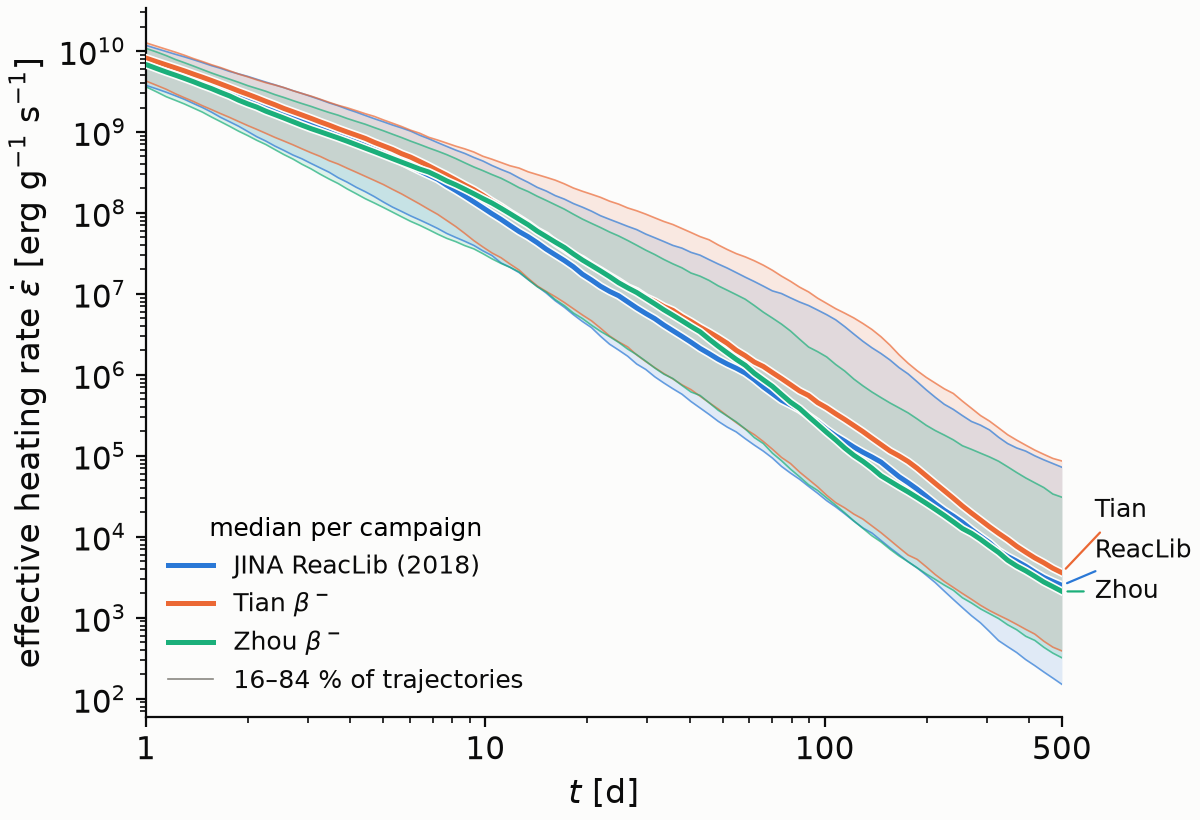
\includegraphics[width=0.7\textwidth]{Figures/heating_bands_sets_therm.png}
  \caption{Median and spread of the total effective heating rate over the 512 trajectories, for each prescription.}
  \label{fig:heating}
\end{figure}
This suggests that the decay channel that dominates the heating depends on the trajectory.
We already saw this behaviour in Chapter~\ref{ch:methods}, in the evolution of $Y_e$ for some trajectories: a low electron fraction combined with a very high velocity favours free neutrons over heavy nuclei, and therefore the $\beta^-$ decay of these neutrons.
We therefore grouped the trajectories by the similarity\footnote{The classification uses Ward hierarchical clustering.} of the time dependence of their ratios $\dot\varepsilon_x/\dot\varepsilon_{\rm total}$ in the three prescriptions, which gives the five classes of Table~\ref{tab:res_classes}.
Figure~\ref{fig:res_class_map} shows where they lie in the parameter space.

\begin{figure}[H]
  \centering
  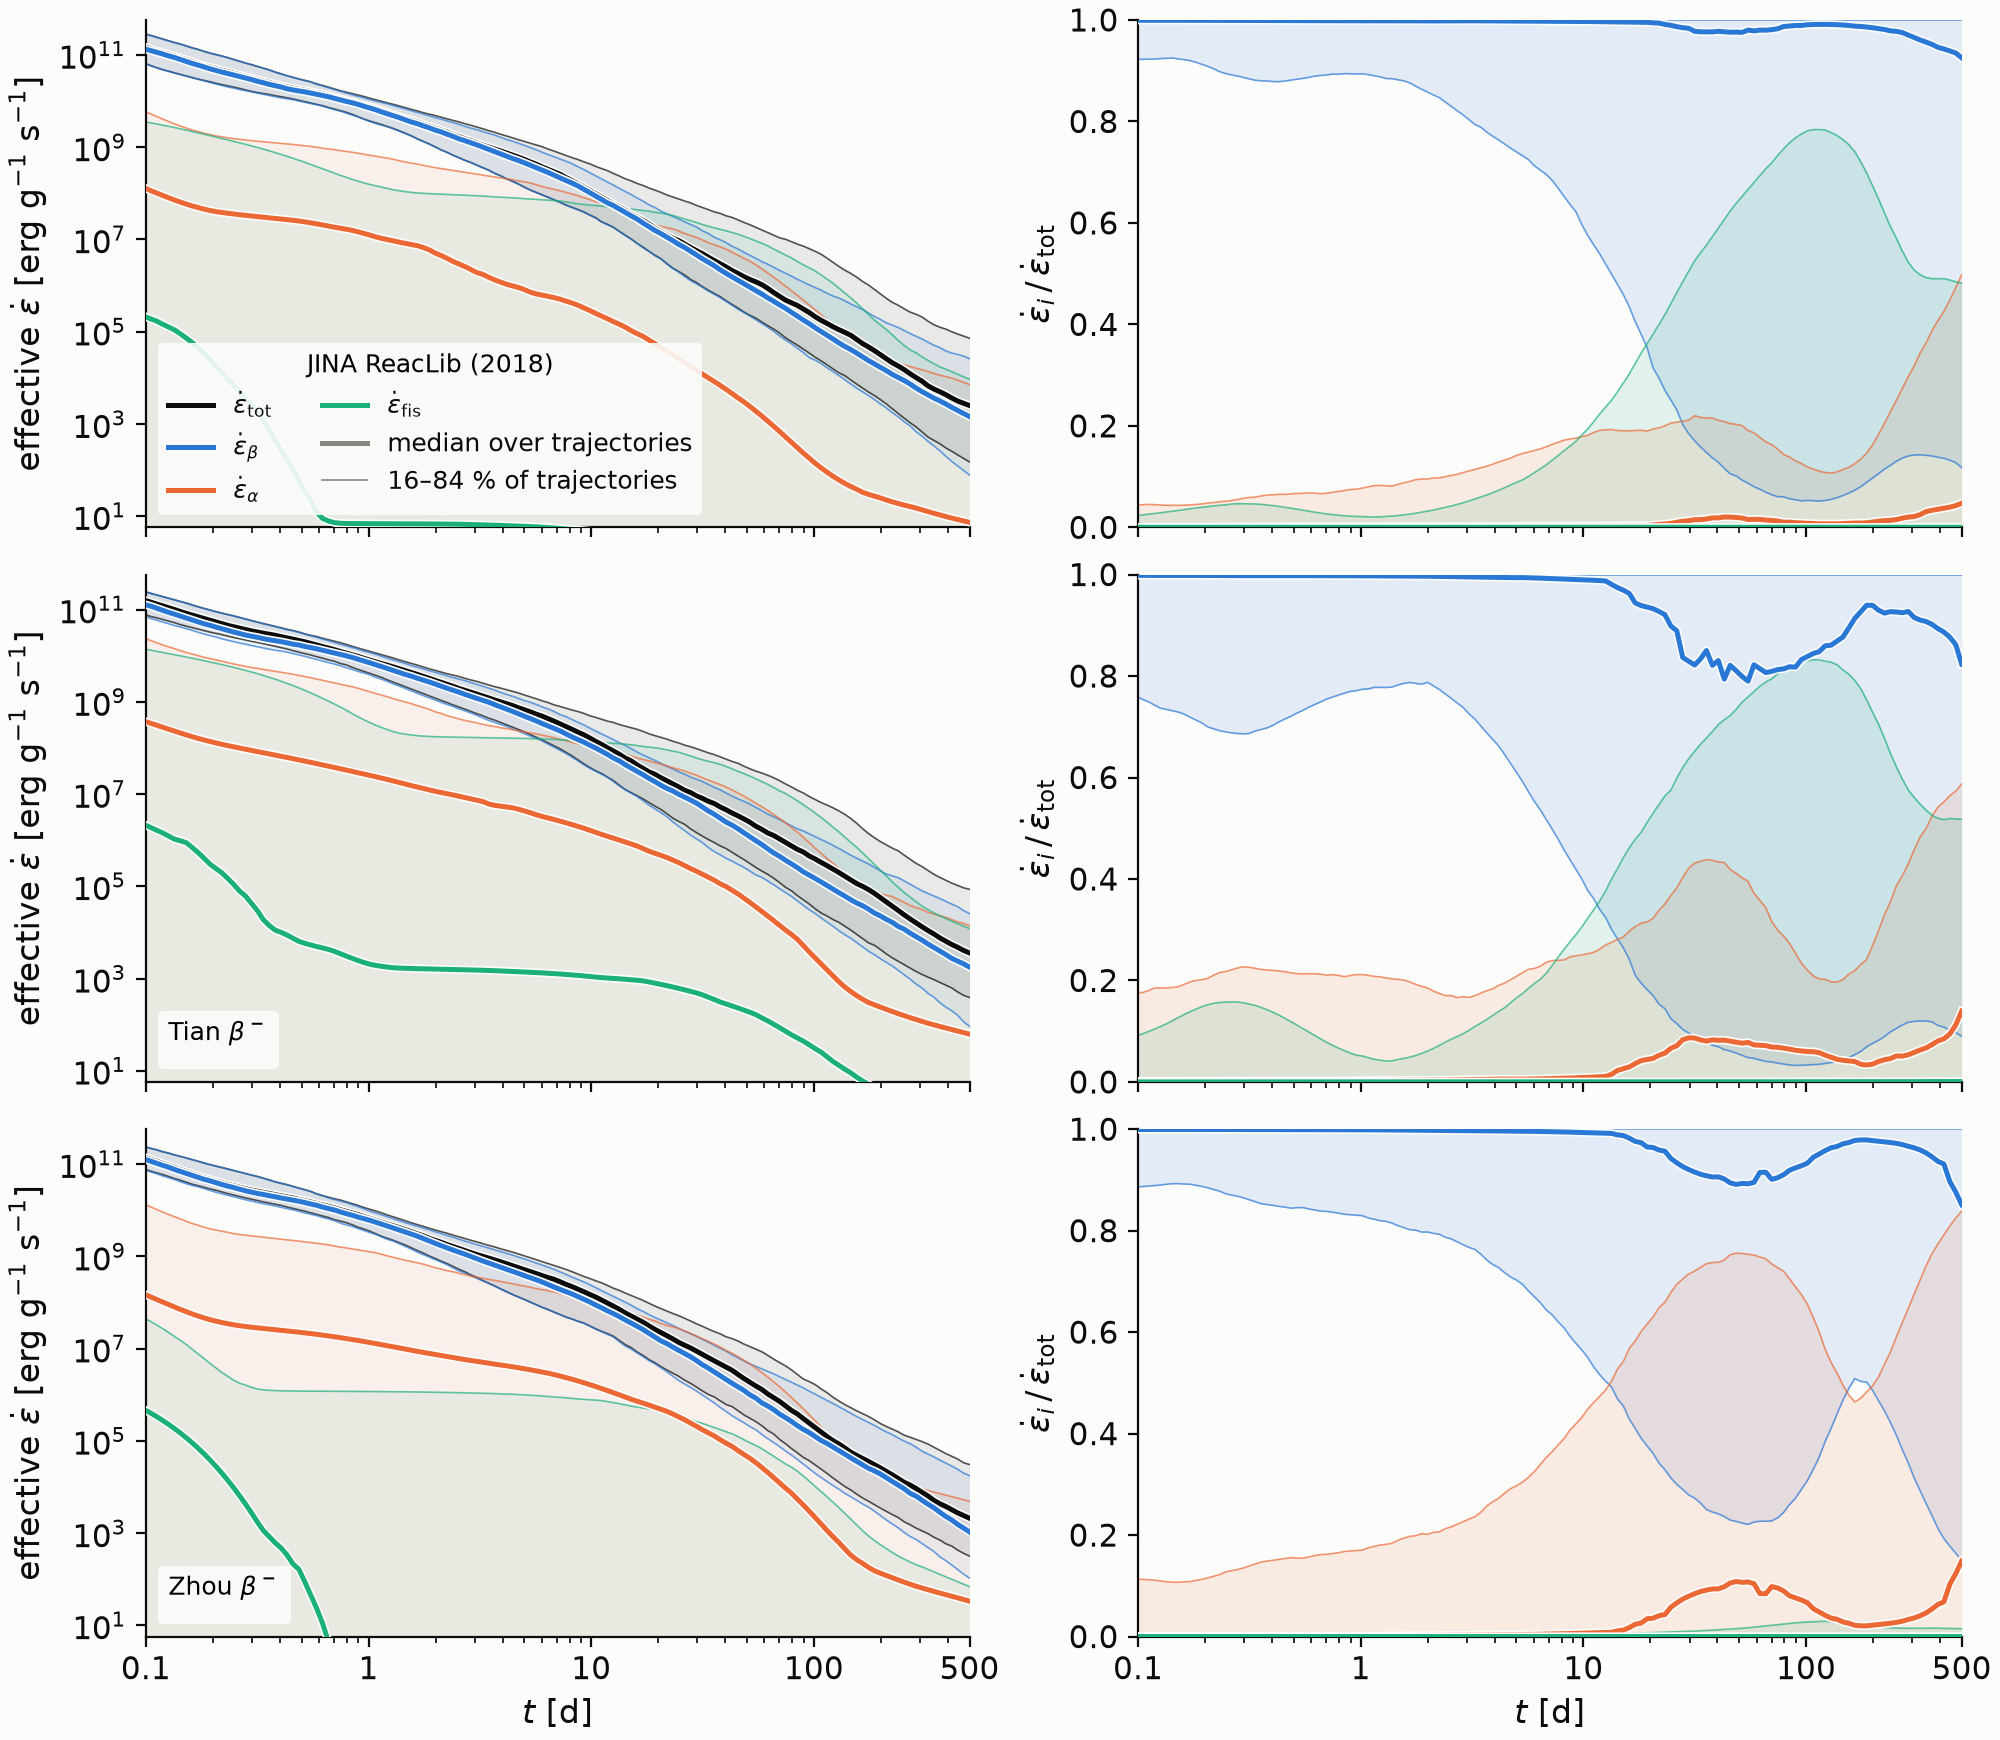
\includegraphics[width=0.8\textwidth]{Figures/heating_channels_sets_therm.png}
  \caption{Median and spread of the total, $\alpha$, $\beta^-$ and fission effective heating rates over the 512 trajectories, for each prescription.}
  \label{fig:heating_chanels}
\end{figure}

\begin{table}[H]
\caption{Classes of trajectories. For each parameter the median and, in brackets, the 16th and 84th percentiles over the class are given.\label{tab:res_classes}}\vspace{0.25em}
\centering{\footnotesize
\begin{tabular}{@{}crccc@{}}
\toprule
Class & $N$ & $Y_{e,0}$ & $s_0\ [k_B]$ & $v_\infty/c$ \\
\midrule
1 & 264 & $0.32\,[0.25, 0.39]$ & $22\,[8, 39]$ & $0.26\,[0.09, 0.42]$ \\
2 & 87 & $0.12\,[0.07, 0.16]$ & $17\,[5, 35]$ & $0.14\,[0.05, 0.31]$ \\
3 & 68 & $0.10\,[0.06, 0.16]$ & $37\,[26, 46]$ & $0.38\,[0.27, 0.45]$ \\
4 & 47 & $0.13\,[0.07, 0.18]$ & $29\,[17, 42]$ & $0.25\,[0.16, 0.36]$ \\
5 & 46 & $0.21\,[0.18, 0.25]$ & $21\,[5, 40]$ & $0.17\,[0.04, 0.33]$ \\
\bottomrule
\end{tabular}}
\end{table}

%%%%%%%%%%%%%%%%%  figure: class map  %%%%%%%%%%%%%%%%%
\begin{figure}[H]
  \centering
  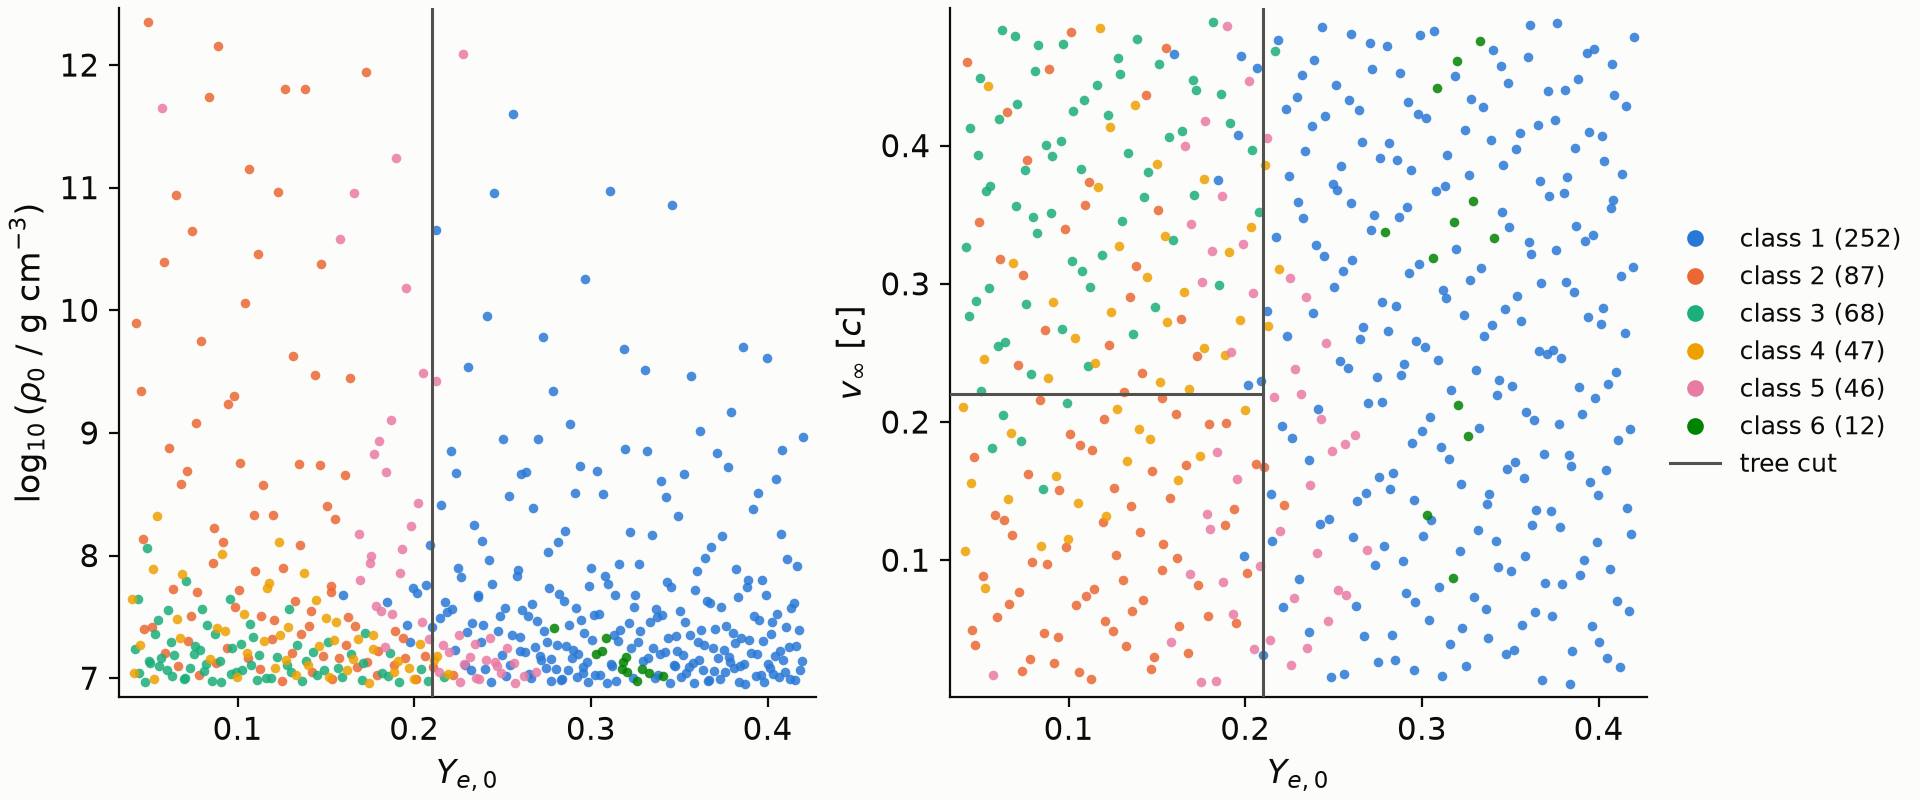
\includegraphics[width=\textwidth]{Figures/ratio_classes_map.png}
  \caption{Projections of the ensemble on the coordinate planes of the parameter space, coloured by class. The dashed lines mark $Y_{e,0}=0.21$ and $v_\infty=0.22\,c$.}
  \label{fig:res_class_map}
\end{figure}

The classes are organized mainly by the electron fraction and, within it, by the expansion.
Class~1 contains half of the box.
Of its 264 trajectories, 255 have $Y_{e,0}\geq0.21$, but it extends down to $Y_{e,0}=0.16$ for intermediate entropies and fast expansions, so $Y_{e,0}$ alone does not decide whether a trajectory belongs to a certain class.
Classes~2, 4 and~3 contain the neutron-rich trajectories, $Y_{e,0}\lesssim0.22$, and follow each other along the direction of increasing entropy and decreasing expansion timescale.
This is the direction in which the number of seeds decreases (Eq.~\ref{eq:seed_scaling}) and in which the time available for the flow of matter through the closed shells becomes shorter.
Class~5 straddles $Y_{e,0}\approx0.21$ so it is a transition.
Although there are five classes, two cuts, $Y_{e,0}=0.21$ and $v_\infty=0.22\,c$, reproduce the location of the three large ones, which contain the relevant physical conditions: high electron fraction (class~1), and low electron fraction with low (class~2) or high (class~3) velocity.
Classes~4 and~5 are transitions between them.
Let us analyze the results class by class.

\textit{Class 1:}
In this class the total effective heating rate is dominated by $\beta^-$ decay in all three prescriptions.
The relevant nuclei are the same in the three sets, ${}^{132}$I and ${}^{127}$Sb, which belong to the decay chains
\begin{equation}\label{chain:I132}
  {}^{132}\mathrm{Te}\xrightarrow[3.2 \, {\rm d}] {\beta^{-}}{}^{132}\mathrm{I} \xrightarrow[2.29 \, {\rm h}] {\beta^{-}}{}^{132}\mathrm{Xe}\,\,\,\text{(stable)},
\end{equation}
\begin{equation}\label{chain:Sb127}
  {}^{127}\mathrm{Sb}\xrightarrow[3.8 \, {\rm d}] {\beta^{-}}{}^{127}\mathrm{Te} \xrightarrow[9.35 \, {\rm h}] {\beta^{-}}{}^{127}\mathrm{I}\,\,\,\text{(stable)}.
\end{equation}
The leading heaters are the isobars of the second peak, $A=131$--$133$, together with $A=127$.
These isobars cannot be reached by $\alpha$ decay, and fission is absent.
Therefore, the heating rate is insensitive to the prescription used.
Accordingly, Fig.~\ref{fig:class_1_epsilon_ratios} shows that the three prescriptions give similar total effective heating rates and the shares of the decay channels correspond to just $\beta^{-}$.
\begin{figure}[H]
  \centering
  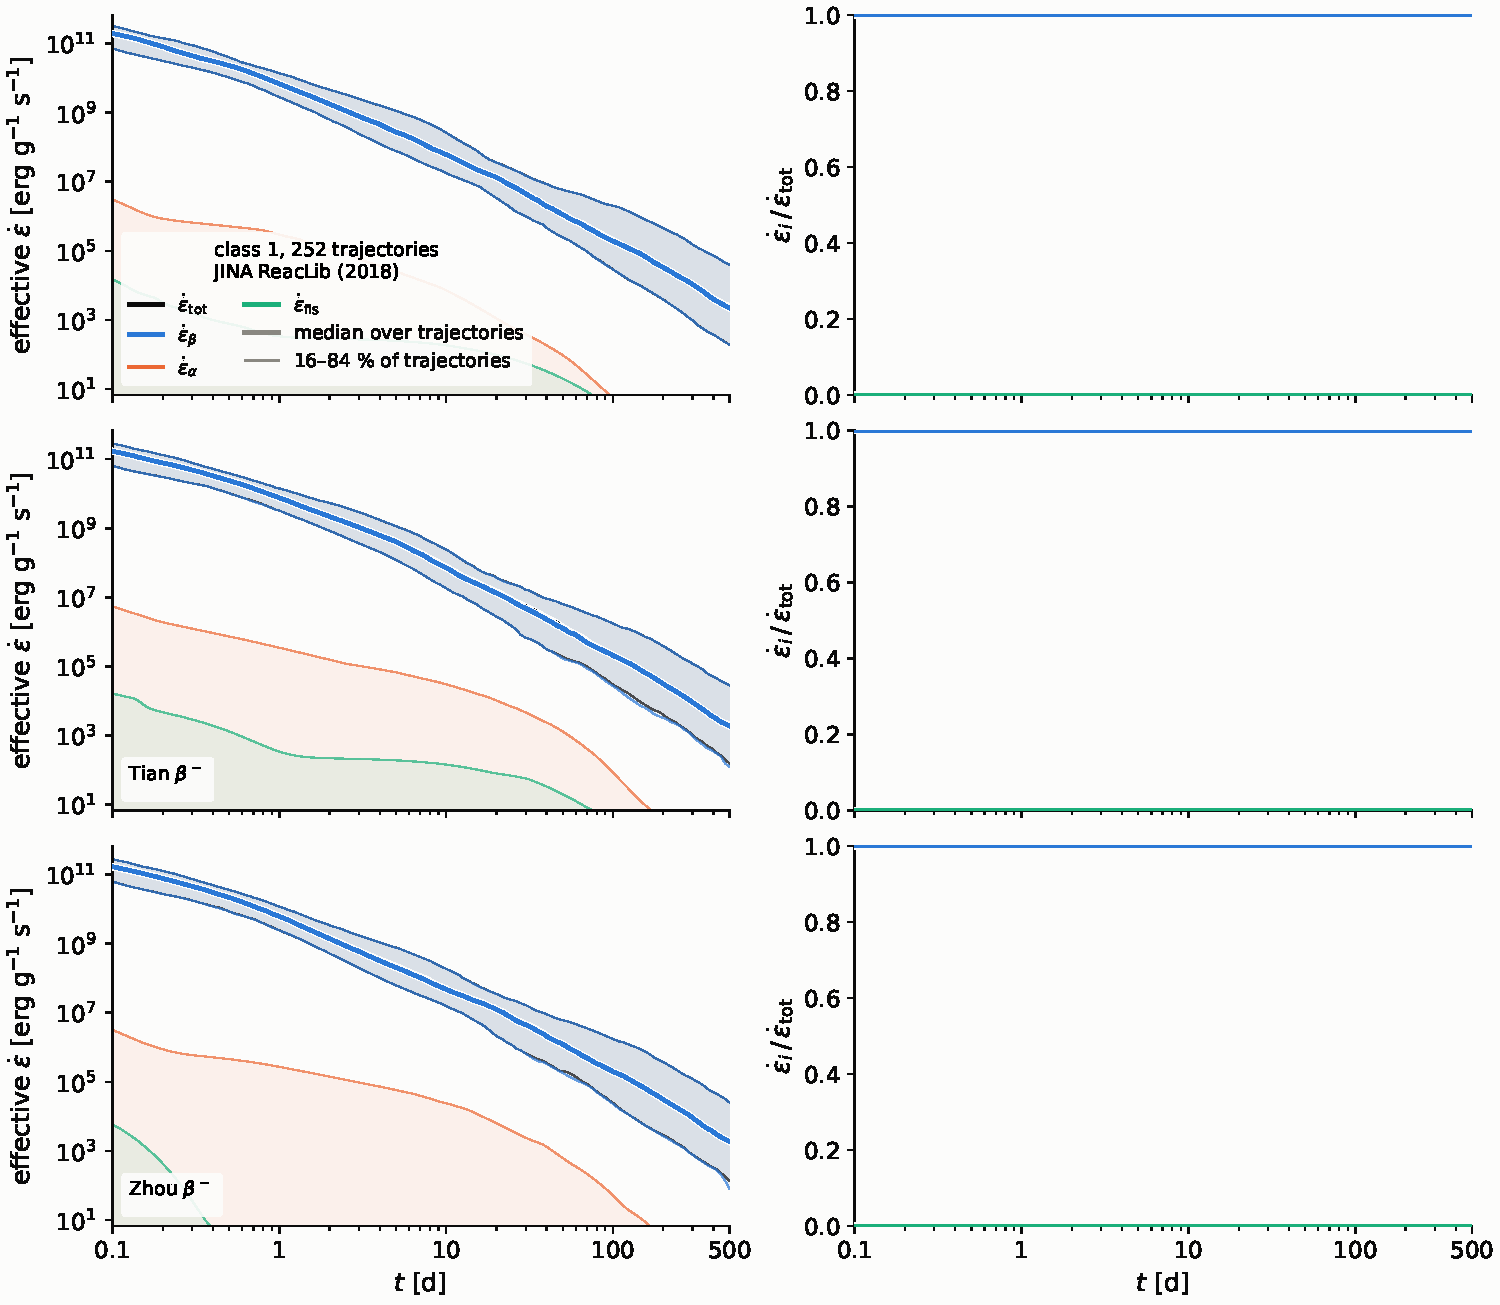
\includegraphics[width=0.8\textwidth]{Figures/heating_channels_sets_therm_class1.pdf}
  \caption{Median and spread of the total, $\alpha$, $\beta^-$ and fission effective heating rates of the trajectories of class~1, for each prescription.}
  \label{fig:class_1_epsilon_ratios}
\end{figure}

\textit{Class 2:}
This class is the slowest (median $v_\infty=0.14\,c$) and contains the neutron-rich trajectories (median $Y_{e,0}=0.12$), the regime of fission cycling (Sec.~\ref{sec:fission}).
It shows the largest differences in the total effective heating rate between prescriptions (Fig.~\ref{fig:class_2_epsilon_ratios_prep}).
At late times the instantaneous ratio between Tian and Zhou is of order 20, and it reaches 40 in some trajectories.
This is not because Tian produces more heating, but because Zhou lacks the fission contribution: fission carries a third of the energy released in Tian and a quarter of that in ReacLib, but only $0.3\%$ of that in Zhou.
The $\alpha$ channel releases a comparable energy in the three sets, but with a different composition.
In ReacLib and Tian it contains the $A\geq240$ emitter ${}^{253}$Es (and, in ReacLib, ${}^{252}$Cf), with the decay chains
\begin{equation}
  {}^{253}\mathrm{Es} \xrightarrow[20.5 \, {\rm d}] {\alpha}{}^{249}\mathrm{Bk} \xrightarrow[327.2 {\rm \, d}] {\beta^-} {}^{249}\mathrm{Cf} \xrightarrow [351 \,{\rm y}] {\alpha} \cdots ,
\end{equation}
\begin{equation}
  {}^{252}\mathrm{Cf} \xrightarrow[2.65 \, {\rm y}] {\alpha}{}^{248}\mathrm{Cm} \xrightarrow[3.48 \times 10^{5} {\rm \, y}] {\alpha} \cdots .
\end{equation}
In Zhou these are absent, and the odd-$A$ series headed by ${}^{225}$Ac and ${}^{223}$Ra dominate:
\begin{equation}
  {}^{225}\mathrm{Ac} \xrightarrow[9.92\,\mathrm{d}]{\alpha}{}^{221}\mathrm{Fr} \xrightarrow[4.8\,\mathrm{min}]{\alpha}{}^{217}\mathrm{At}\cdots,
\end{equation}
\begin{equation}
  {}^{223}\mathrm{Ra} \xrightarrow[11.4 \, {\rm d}] {\alpha}{}^{219}\mathrm{Rn} \xrightarrow[3.96 {\rm \, s}] {\alpha} {}^{215}\mathrm{Po}\cdots.
\end{equation}
The $A\geq240$ material releases its energy mainly by spontaneous fission, 10--18 times more than through the $\alpha$ decays of ${}^{253}$Es and ${}^{252}$Cf.
Since Tian and Zhou share the $\alpha$ rates, the absence of late-time fission in Zhou is an effect of the $\beta^-$ rates.

\begin{figure}[H]
  \centering
  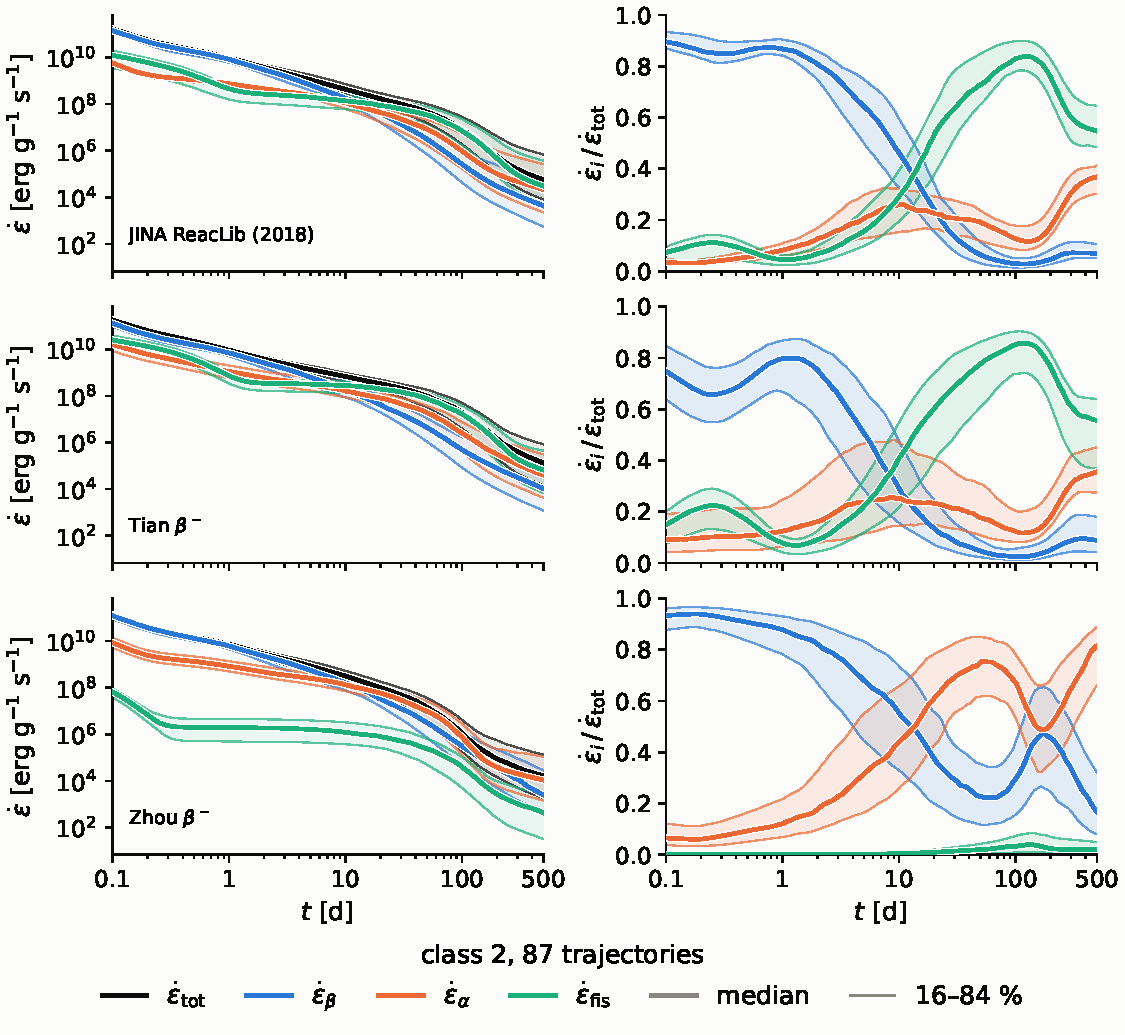
\includegraphics[width=0.8\textwidth]{Figures/heating_channels_sets_therm_class2.pdf}
  \caption{Median and spread of the total, $\alpha$, $\beta^-$ and fission effective heating rates of the trajectories of class~2, for each prescription.}
  \label{fig:class_2_epsilon_ratios}
\end{figure}
\begin{figure}[H]
  \centering
  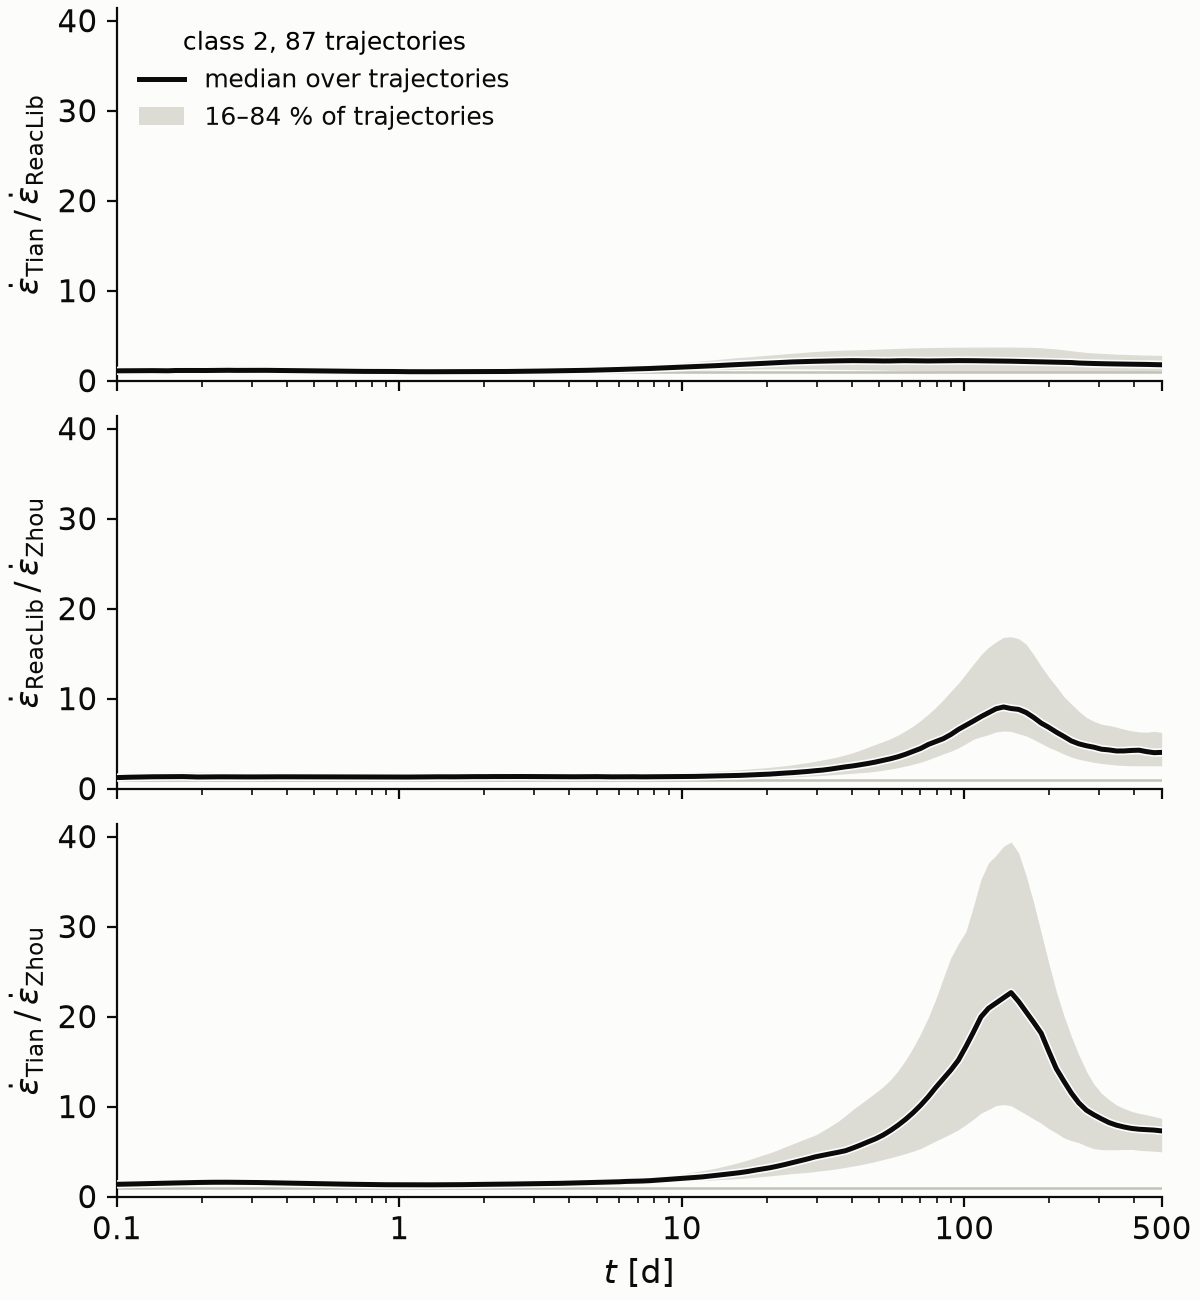
\includegraphics[width=0.5\textwidth]{Figures/heating_ratios_sets_therm_class2.png}
  \caption{Median and spread of the ratio of the effective heating rates between prescriptions, for the trajectories of class~2.}
  \label{fig:class_2_epsilon_ratios_prep}
\end{figure}

\textit{Class 3:}
This class collects the fastest (median $v_\infty=0.38\,c$) and highest-entropy (median $s_0=37$) neutron-rich trajectories, which also have the lowest initial densities.
Under these conditions part of the neutrons are not captured, and their decay produces a rapid increase of $Y_e$ on the timescale of the free-neutron half-life (Fig.~\ref{fig:trajectories_T_Ye}).
No set produces appreciable late-time fission (Fig.~\ref{fig:class_3_epsilon_ratios}).

The empirical sets release more energy than ReacLib (Fig.~\ref{fig:class_3_epsilon_ratios_prep}).
Tian and Zhou agree in the $\alpha$ channel, whereas ReacLib lacks the peak of the $\alpha$ share between 10 and 100\,d.
The $\alpha$ decay chain that appears in all prescriptions is
\begin{equation}
  {}^{224}\mathrm{Ra} \xrightarrow[3.63 \, {\rm d}] {\alpha}{}^{220}\mathrm{Rn} \xrightarrow[55.6 {\rm \, s}] {\alpha} {}^{216}\mathrm{Po}\xrightarrow[144 {\rm \, ms}] {\alpha} {}^{212}\mathrm{Pb}\xrightarrow[10.6 {\rm \, h}] {\beta^{-}} {}^{212}\mathrm{Bi}.
\end{equation}
${}^{212}$Bi has two decay branches, $\beta^-$ decay to ${}^{212}$Po and $\alpha$ decay to ${}^{208}$Tl, and both end in ${}^{208}$Pb.
The main difference between the prescriptions is that Zhou and Tian also have a contribution from the odd-$A$ chain
\begin{equation}
    {}^{223}\mathrm{Ra} \xrightarrow[11.4 \, {\rm d}] {\alpha}{}^{219}\mathrm{Rn} \xrightarrow[3.96 {\rm \, s}] {\alpha} {}^{215}\mathrm{Po}\xrightarrow[1.78 {\rm \, ms}] {\alpha} {}^{211}\mathrm{Pb}\xrightarrow[36.1 {\rm \, min}] {\beta^{-}} {}^{211}\mathrm{Bi}\xrightarrow[2.1 {\rm \, min}] {\alpha} {}^{207}\mathrm{Tl}\xrightarrow[4.77 {\rm \, min}] {\beta^{-}} {}^{207}\mathrm{Pb}\,\,\text{(stable)}.
\end{equation}

Notice that the abundance of ${}^{224}$Ra feeds on the $\beta^{-}$ decay of ${}^{224}$Fr (half-life$\sim 3\,\mathrm{min}$) and on the $\alpha$ decay of ${}^{228}$Th (half-life$\sim 2\,\mathrm y$) which means that ${}^{224}$Ra contributes at large times as ${}^{228}$Th decays.
On the other hand, the time scale of the contribution of ${}^{225}$Ac and ${}^{223}$Ra is around $\sim10\,\mathrm d$.
\begin{figure}[H]
  \centering
  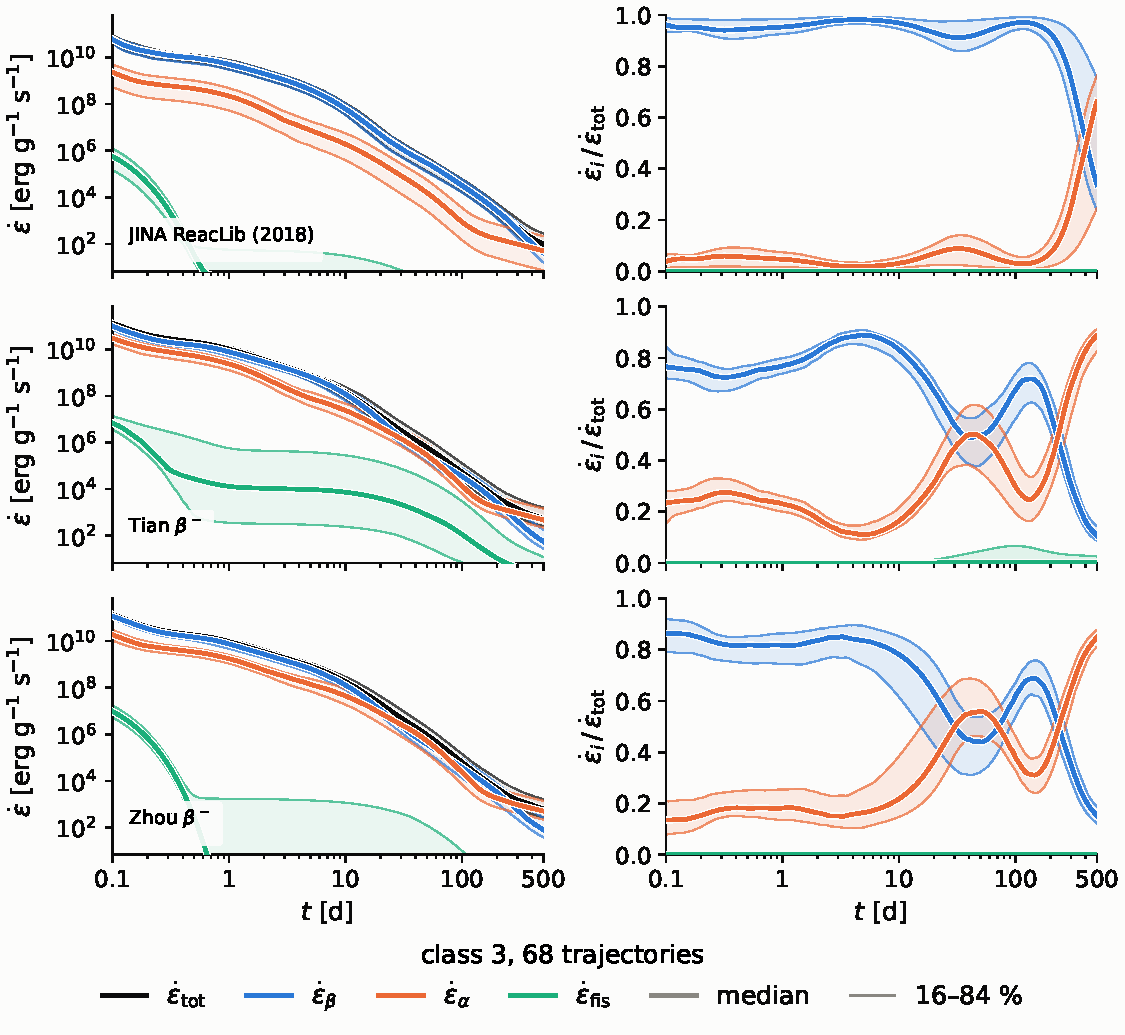
\includegraphics[width=0.8\textwidth]{Figures/heating_channels_sets_therm_class3.pdf}
  \caption{Median and spread of the total, $\alpha$, $\beta^-$ and fission effective heating rates of the trajectories of class~3, for each prescription.}
  \label{fig:class_3_epsilon_ratios}
\end{figure}
\begin{figure}[H]
  \centering
  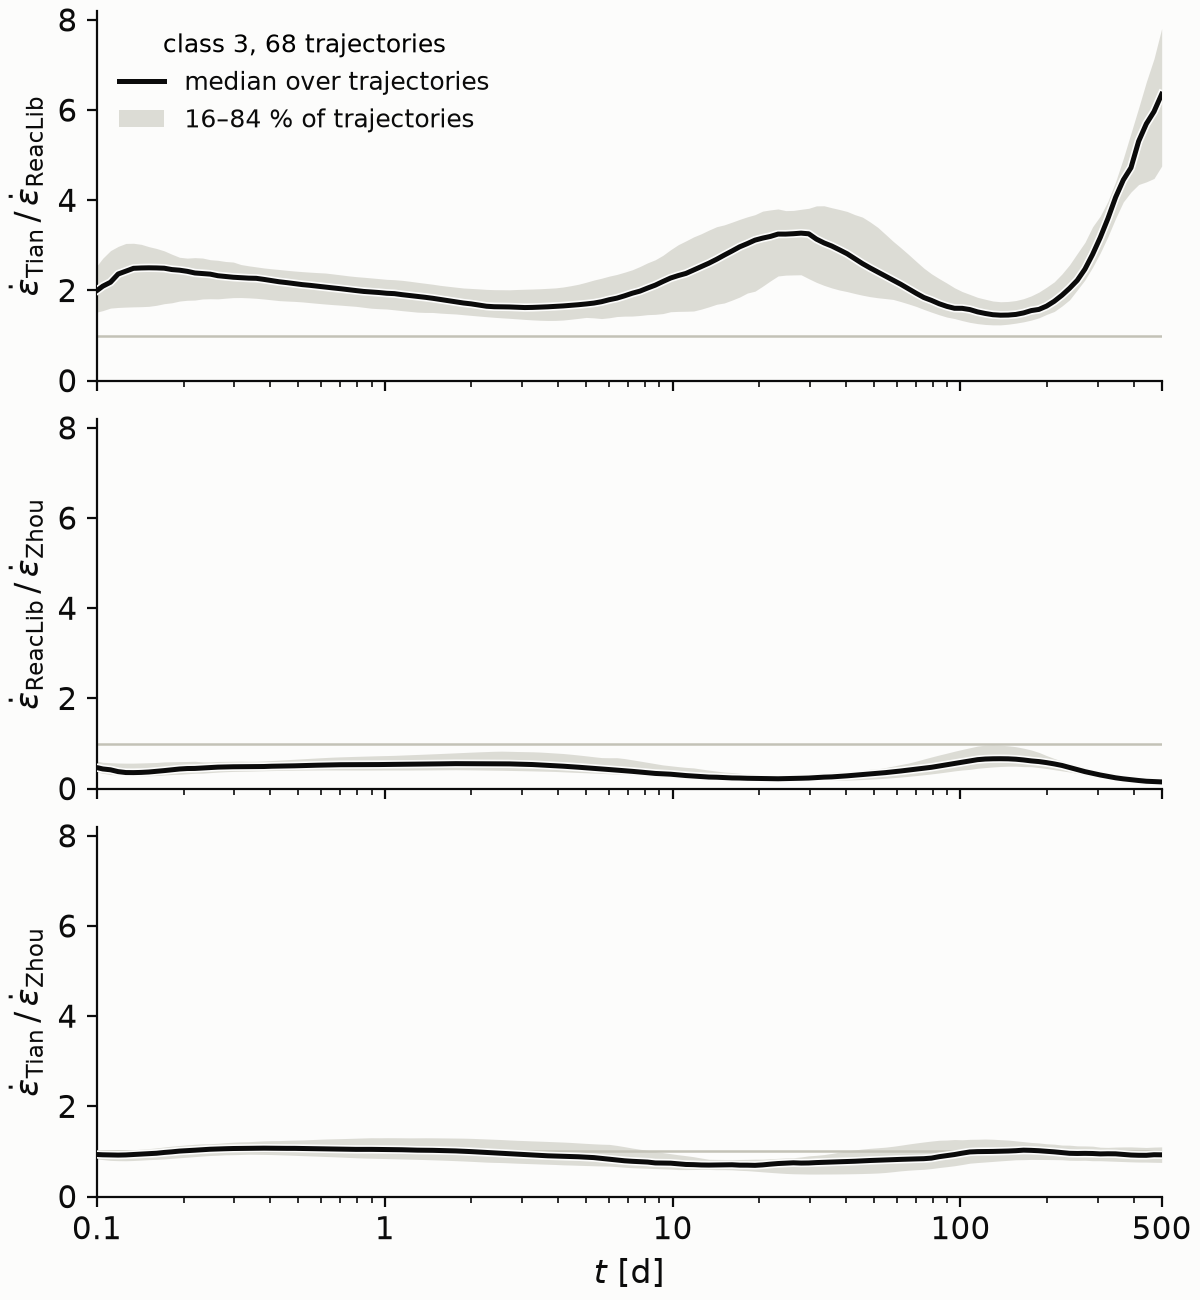
\includegraphics[width=0.6\textwidth]{Figures/heating_ratios_sets_therm_class3.png}
  \caption{Median and spread of the ratio of the effective heating rates between prescriptions, for the trajectories of class~3.}
  \label{fig:class_3_epsilon_ratios_prep}
\end{figure}
%--------------------------------------------------------------------
\textit{Class 4:}
This class lies between classes~2 and~3 (median $s_0=29$, $v_\infty=0.25\,c$), and here each set heats through a different combination of channels.
ReacLib heats almost only by $\beta^-$ decay, half of it in the isobar $A=202$ (${}^{202}$Pt$\to{}^{202}$Au) on the high-mass side of the third peak.
Tian adds fission and $\alpha$ decay, whereas Zhou adds only $\alpha$ decay, carried by the odd-$A$ series.
Figure~\ref{fig:class_4_epsilon_ratios_prep} shows that Tian has a higher total effective heating rate than ReacLib, mainly because of fission, while Zhou has a larger contribution from $\alpha$ decay.
In this class, therefore, each prescription has its own preferred decay channel.
\begin{figure}[H]
  \centering
  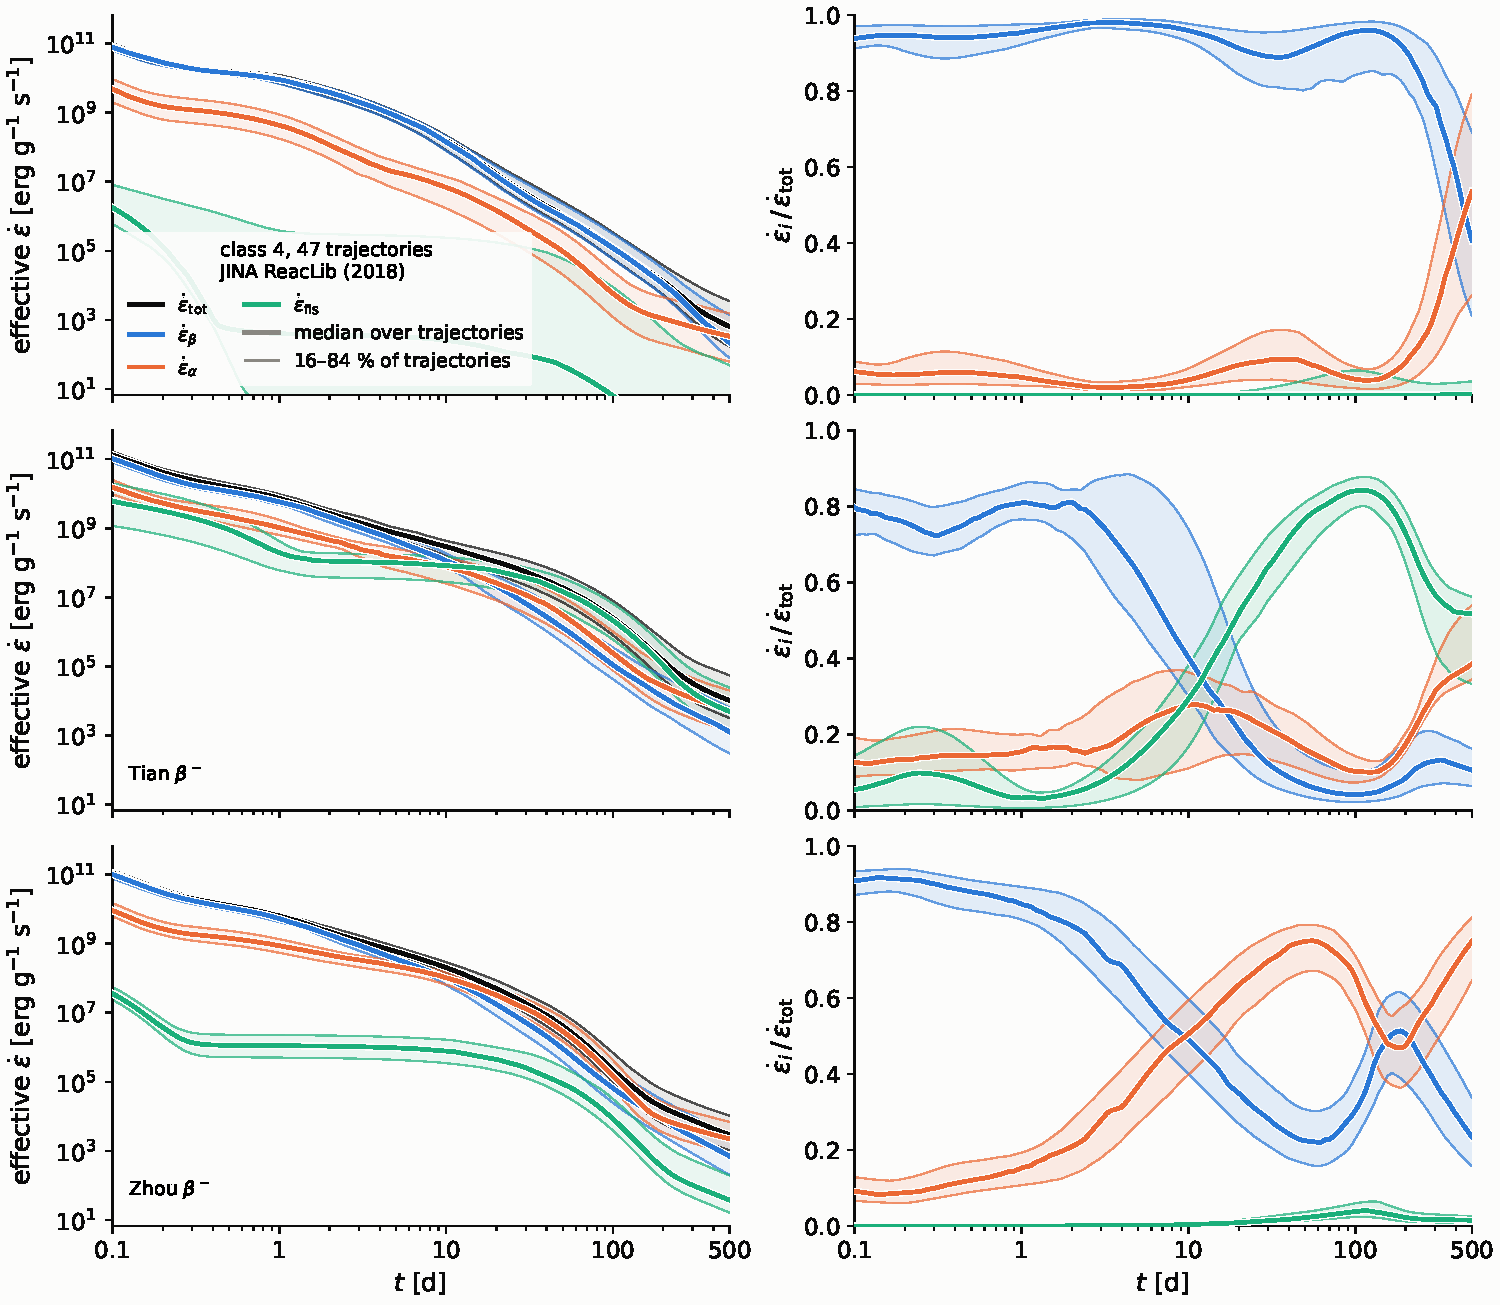
\includegraphics[width=0.8\textwidth]{Figures/heating_channels_sets_therm_class4.pdf}
  \caption{Median and spread of the total, $\alpha$, $\beta^-$ and fission effective heating rates of the trajectories of class~4, for each prescription.}
  \label{fig:class_4_epsilon_ratios}
\end{figure}
\begin{figure}[H]
  \centering
  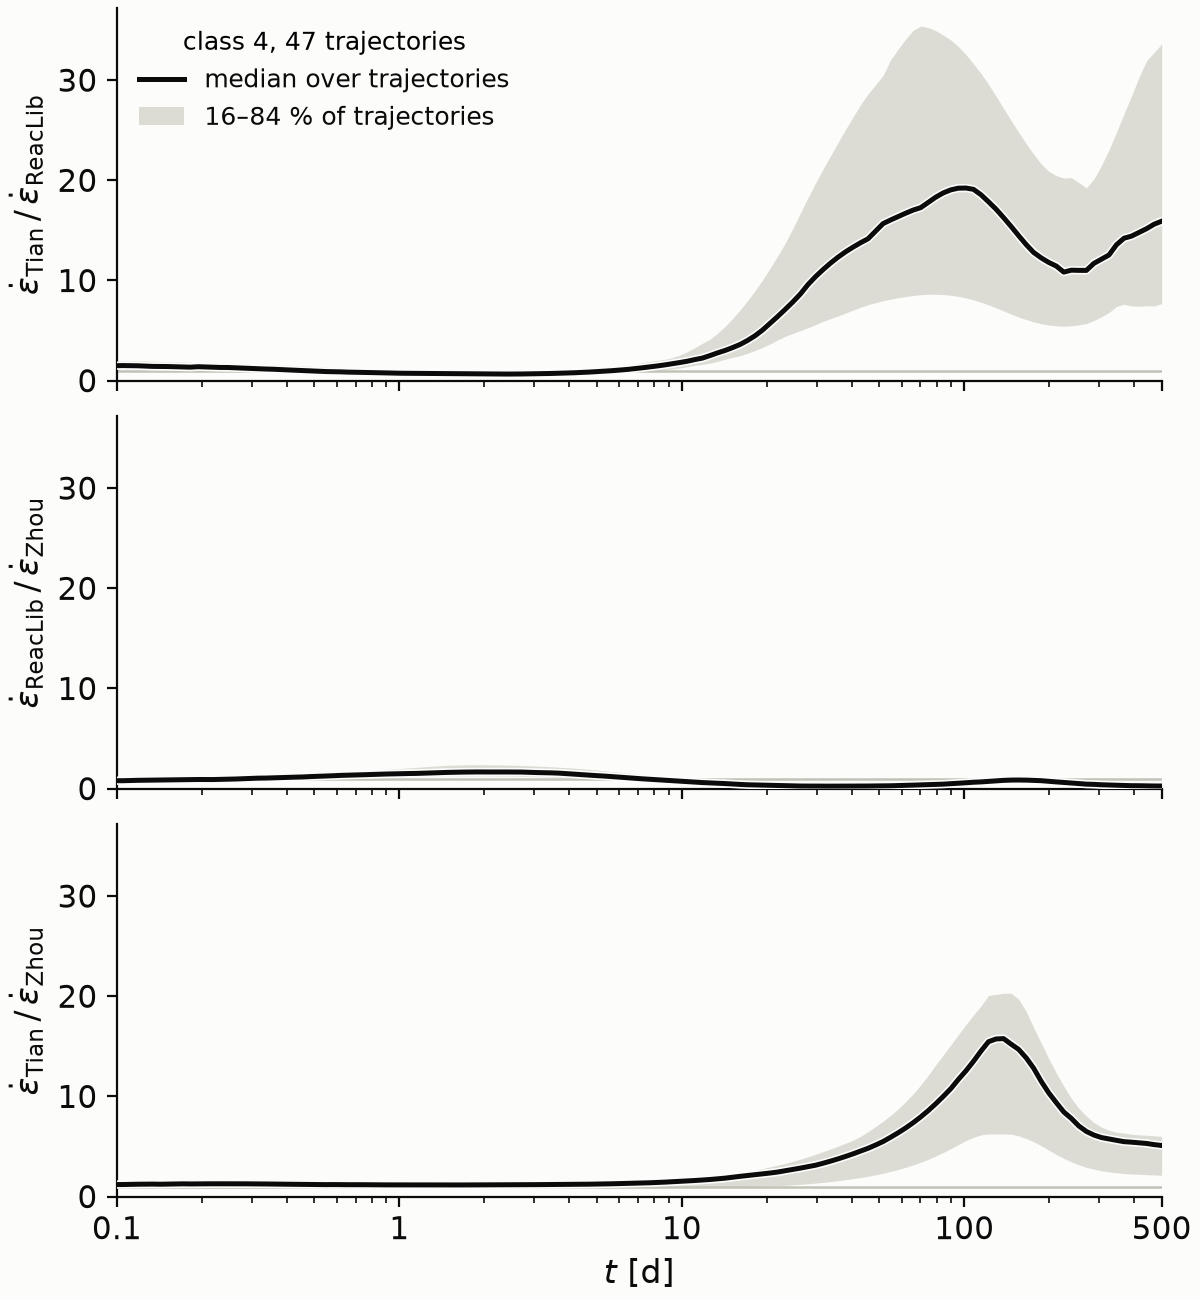
\includegraphics[width=0.6\textwidth]{Figures/heating_ratios_sets_therm_class4.png}
  \caption{Median and spread of the ratio of the effective heating rates between prescriptions, for the trajectories of class~4.}
  \label{fig:class_4_epsilon_ratios_prep}
\end{figure}

\textit{Class 5:}
This class lies at $Y_{e,0}\approx0.21$ and spans the full range of entropies and velocities.
It is a transition between class~1, heated only by $\beta^-$ decay, and classes~2, 3 and~4.
The main difference between the prescriptions is between Zhou and ReacLib: ReacLib has a fission contribution at late times, whereas Zhou does not.
\begin{figure}[H]
  \centering
  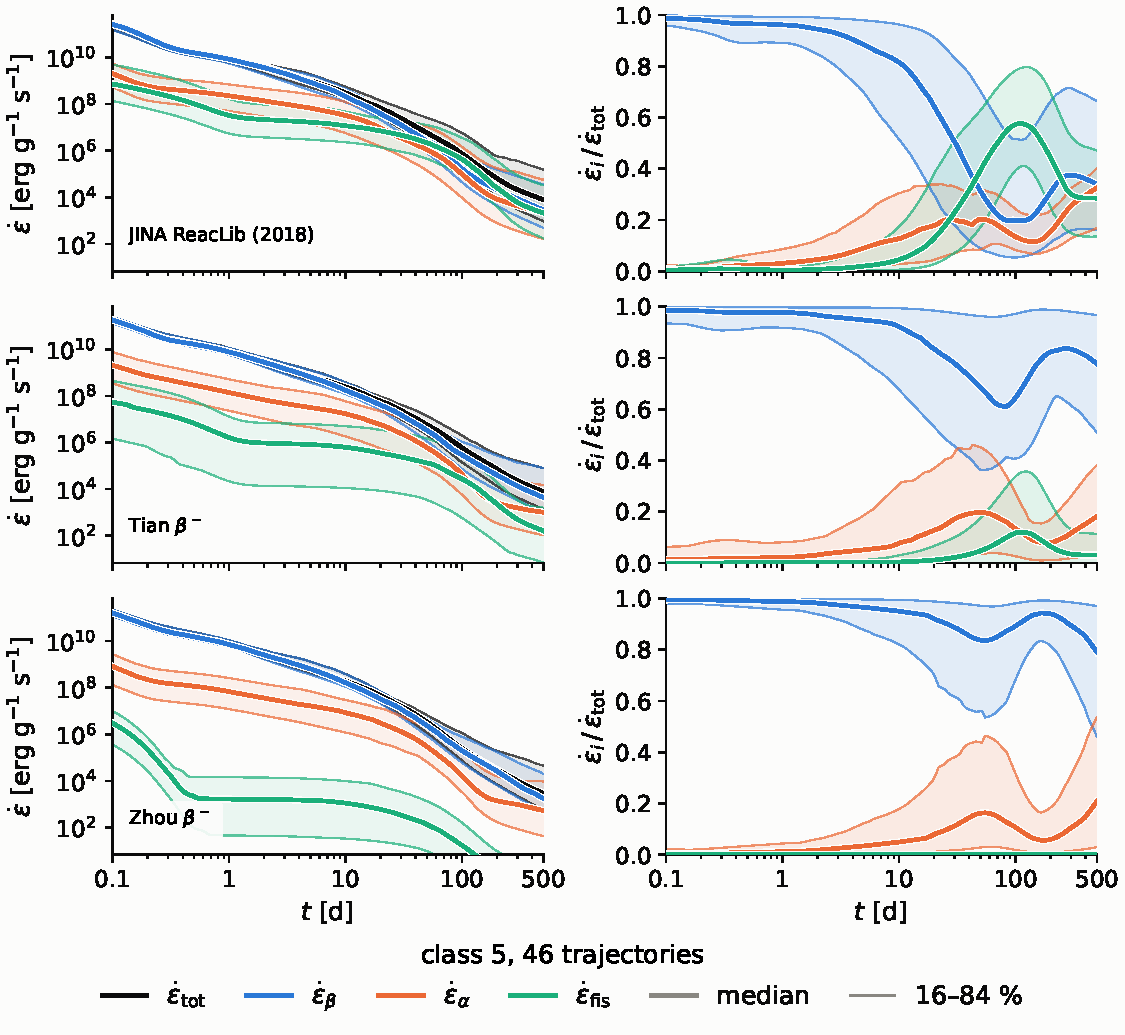
\includegraphics[width=0.8\textwidth]{Figures/heating_channels_sets_therm_class5.pdf}
  \caption{Median and spread of the total, $\alpha$, $\beta^-$ and fission effective heating rates of the trajectories of class~5, for each prescription.}
  \label{fig:class_5_epsilon_ratios}
\end{figure}
\begin{figure}[H]
  \centering
  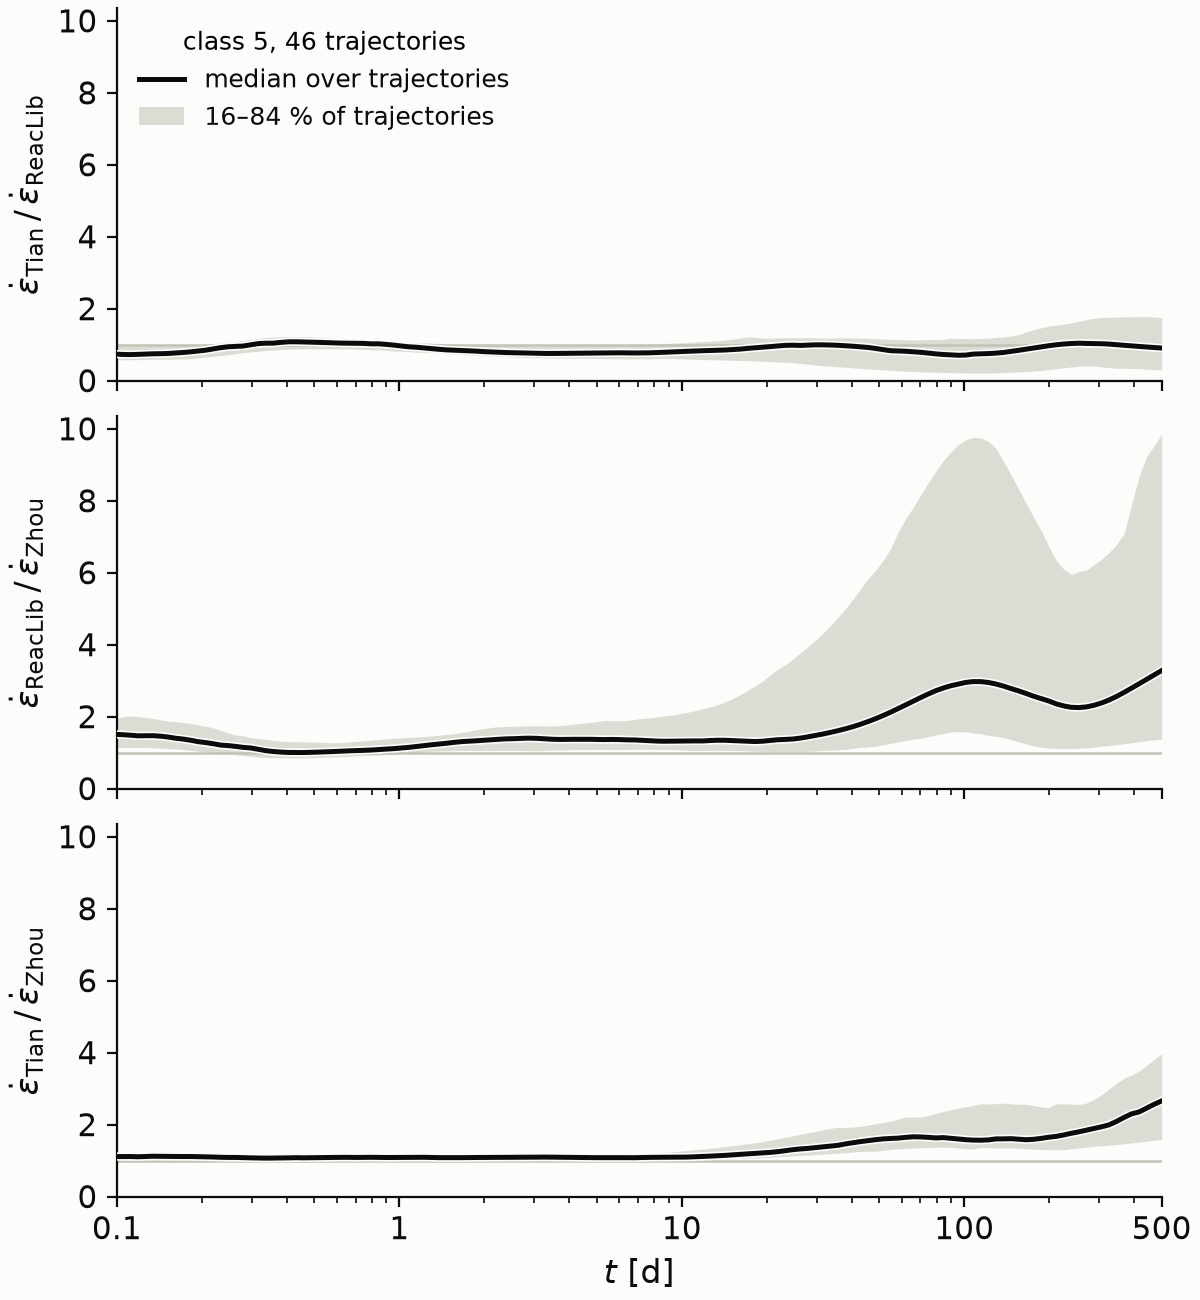
\includegraphics[width=0.6\textwidth]{Figures/heating_ratios_sets_therm_class5.png}
  \caption{Median and spread of the ratio of the effective heating rates between prescriptions, for the trajectories of class~5.}
  \label{fig:class_5_epsilon_ratios_prep}
\end{figure}

%--------------------------------------------------------------------
\subsection{Where these conditions occur in a merger}\label{sec:res_merger}

The ensemble is a uniform design over a box, not a model of a particular merger (Sec.~\ref{sec:methods_sampling}).
Each class can nevertheless be related to the ejecta components of Chapter~\ref{chap:BNMS}, which indicates where in a merger each behaviour would appear.
Simulations find that most of the dynamical ejecta moves at $0.1$--$0.3\,c$, with an electron fraction that increases from the orbital plane, where the cold tidal ejecta have $Y_e\lesssim0.15$, towards the poles, where shock heating and neutrino irradiation raise it up to $Y_e\approx0.4$~\cite{radice_binary_2018,radice_dynamics_2020}.
A small amount of matter from the collision interface is accelerated to $v\gtrsim0.4$--$0.6\,c$, and it expands so fast that part of its neutrons are never captured~\cite{metzger_neutron-powered_2015,metzger_kilonovae_2017}.
The outflows from the post-merger torus are slower, $v\approx0.03$--$0.1\,c$, with $Y_e\approx0.1$--$0.25$ when the remnant collapses early to a black hole~\cite{fernandez_long-term_2019}, and with higher $Y_e$ when they are irradiated by the neutrinos of a long-lived neutron star~\cite{metzger_kilonovae_2017}.
Table~\ref{tab:res_merger} places the classes in this picture.

\begin{table}[h]
\caption{Merger components with conditions similar to those of each class.\label{tab:res_merger}}\vspace{0.25em}
\centering{\small
\begin{tabular}{@{}cp{0.3\textwidth}p{0.55\textwidth}@{}}
\toprule
Class & Conditions & Merger component\\
\midrule
1 & $Y_{e,0}\gtrsim0.21$, all velocities & Shock-heated and neutrino-irradiated dynamical ejecta at high latitudes; for $v\lesssim0.1\,c$, outflows irradiated by a long-lived remnant\\
2 & $Y_{e,0}\lesssim0.16$, slow & Cold tidal ejecta near the orbital plane; neutron-rich outflows of a torus around an early black hole\\
3 & $Y_{e,0}\lesssim0.16$, fast, high entropy, low density & Fast outer layers of the dynamical ejecta, from the collision interface\\
4 & $Y_{e,0}\lesssim0.18$, intermediate entropy and velocity & Shock-heated dynamical ejecta at low latitudes, not reprocessed by neutrinos\\
5 & $Y_{e,0}\approx0.18$--$0.25$ & Intermediate latitudes; less neutron-rich part of the torus outflows\\
\bottomrule
\end{tabular}}
\end{table}

Two remarks are needed.
First, the classes do not carry comparable masses in a real merger.
Class~3 is 13\% of the box, but the fast matter that it represents amounts to at most $\sim10^{-4}\,M_\odot$, and to $10^{-6}$--$10^{-5}\,M_\odot$ for $v>0.6\,c$ in high-resolution simulations~\cite{metzger_neutron-powered_2015,radice_binary_2018}.
In a merger, class-3 conditions are restricted to the outermost layers, where the free neutrons would power an hour-long precursor rather than the main kilonova~\cite{metzger_neutron-powered_2015}.
Most of the mass is instead expected in classes~1, 2, 4 and~5.
Second, which of these classes dominates depends on the binary: the tidal ejecta dominate for unequal masses and stiff equations of state, the shock-heated ejecta for equal masses and soft ones (Chapter~\ref{chap:BNMS}), and the lifetime of the remnant controls the electron fraction of the torus outflows.
The large sensitivity of classes~2 and~4 is therefore most relevant for asymmetric binaries and for remnants that collapse early, which eject large masses of slow, neutron-rich matter.

%------------------------------------------------------------------------------------------
\section{Final abundances and the origin of the dependence on the decay rates}\label{sec:res_origin}
%------------------------------------------------------------------------------------------

Since the relevant nuclei themselves have measured decays, the differences between the sets are differences in where the matter ends.
Table~\ref{tab:res_abund} and Fig.~\ref{fig:res_abund} show the final composition of the five classes.

\begin{table}[t]
\caption{Mass fractions at 500\,d summed over ranges of mass number, and lanthanide plus actinide mass fraction $X_{\rm LA}$, averaged over the trajectories of each class.\label{tab:res_abund}}\vspace{0.25em}
\centering{\footnotesize
\begin{tabular}{@{}clccccccc@{}}
\toprule
Class & Set & $A<70$ & $70$--$90$ & $120$--$140$ & $150$--$180$ & $185$--$205$ & $A\geq210$ & $X_{\rm LA}$\\
\midrule
1 & ReacLib & 0.11 & 0.24 & 0.29 & 0.015 & 0.030 & $\approx0$ & 0.026\\
  & Tian    & 0.11 & 0.23 & 0.28 & 0.025 & 0.038 & $\approx0$ & 0.036\\
  & Zhou    & 0.11 & 0.23 & 0.27 & 0.033 & 0.035 & $\approx0$ & 0.046\\
\midrule
2 & ReacLib & 0.01 & $\approx0$ & 0.38 & 0.075 & 0.43 & 0.077 & 0.165\\
  & Tian    & 0.01 & $\approx0$ & 0.30 & 0.071 & 0.42 & 0.140 & 0.247\\
  & Zhou    & 0.01 & $\approx0$ & 0.27 & 0.107 & 0.45 & 0.100 & 0.255\\
\midrule
3 & ReacLib & 0.50 & $\approx0$ & 0.10 & 0.019 & 0.34 & 0.002 & 0.029\\
  & Tian    & 0.30 & $\approx0$ & 0.21 & 0.029 & 0.33 & 0.021 & 0.046\\
  & Zhou    & 0.22 & $\approx0$ & 0.28 & 0.051 & 0.31 & 0.028 & 0.083\\
\midrule
4 & ReacLib & 0.11 & $\approx0$ & 0.16 & 0.042 & 0.61 & 0.005 & 0.067\\
  & Tian    & 0.03 & $\approx0$ & 0.21 & 0.090 & 0.53 & 0.056 & 0.174\\
  & Zhou    & 0.03 & $\approx0$ & 0.21 & 0.132 & 0.51 & 0.049 & 0.223\\
\midrule
5 & ReacLib & 0.02 & 0.01 & 0.50 & 0.097 & 0.32 & 0.025 & 0.141\\
  & Tian    & 0.02 & $\approx0$ & 0.43 & 0.145 & 0.35 & 0.009 & 0.179\\
  & Zhou    & 0.02 & $\approx0$ & 0.40 & 0.194 & 0.33 & 0.006 & 0.241\\
\bottomrule
\end{tabular}}
\end{table}

%%%%%%%%%%%%%%%%%  figure: abundances  %%%%%%%%%%%%%%%%%
\begin{figure}[h]
\centering
\subfloat[Class 1]{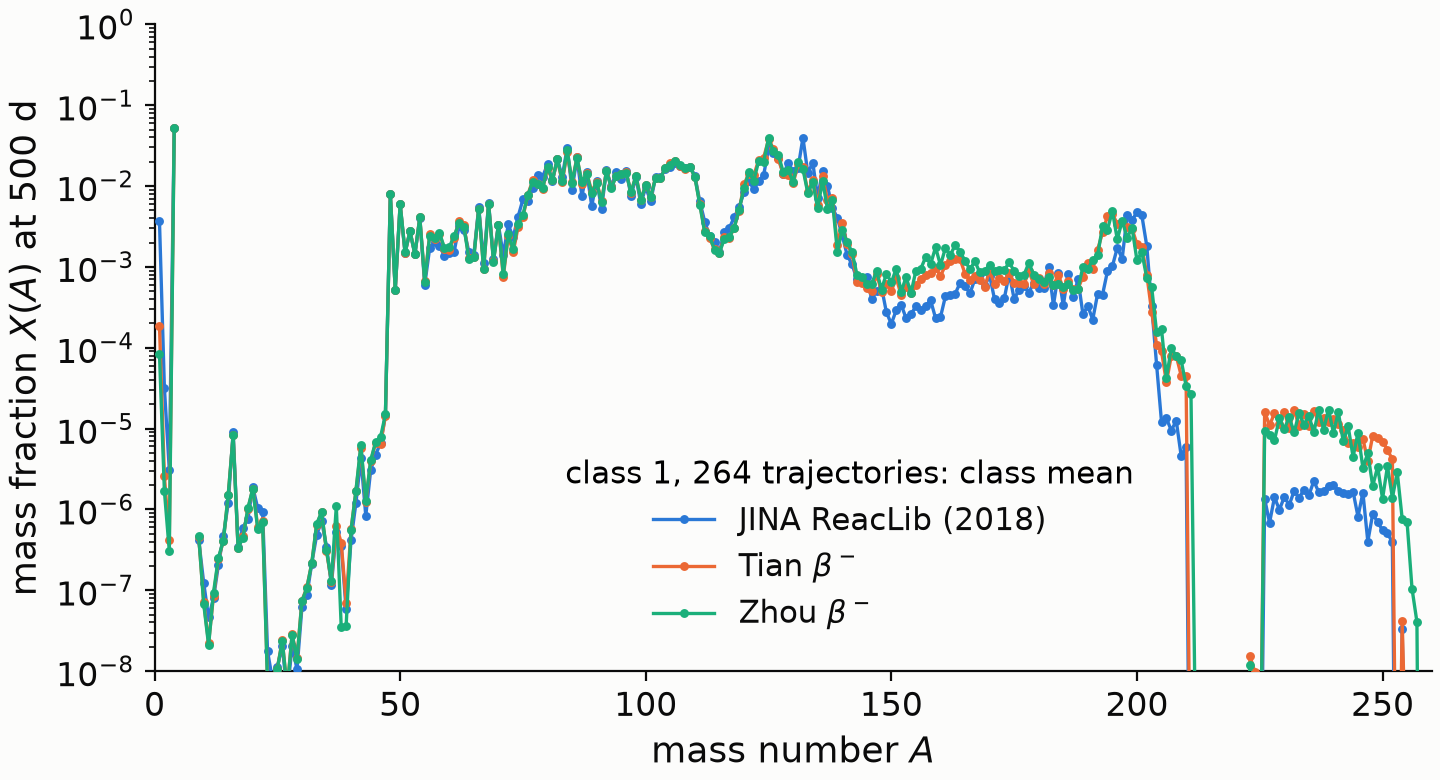
\includegraphics[width=0.5\textwidth]{Figures/abundances_class1.png}}\hfil
\subfloat[Class 2]{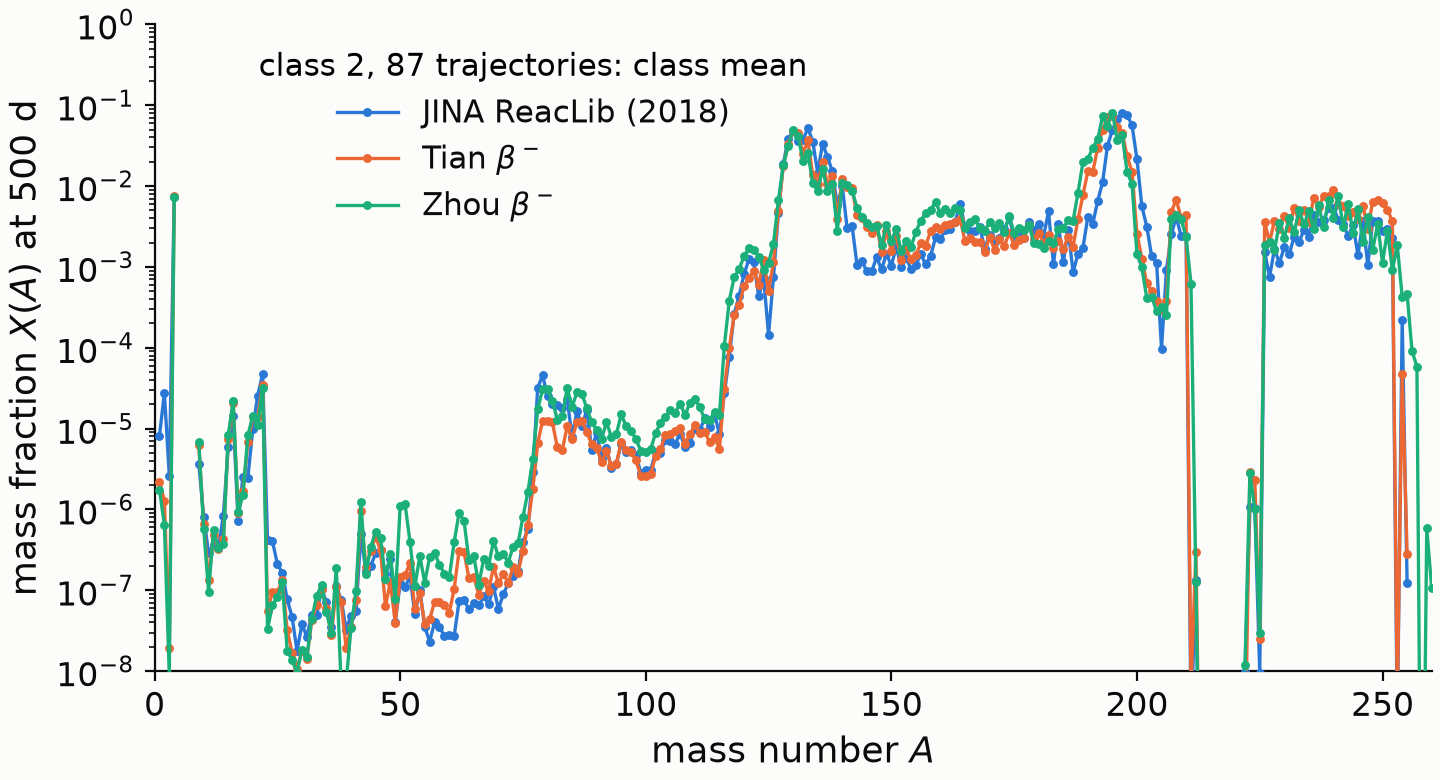
\includegraphics[width=0.5\textwidth]{Figures/abundances_class2.png}}

\subfloat[Class 3]{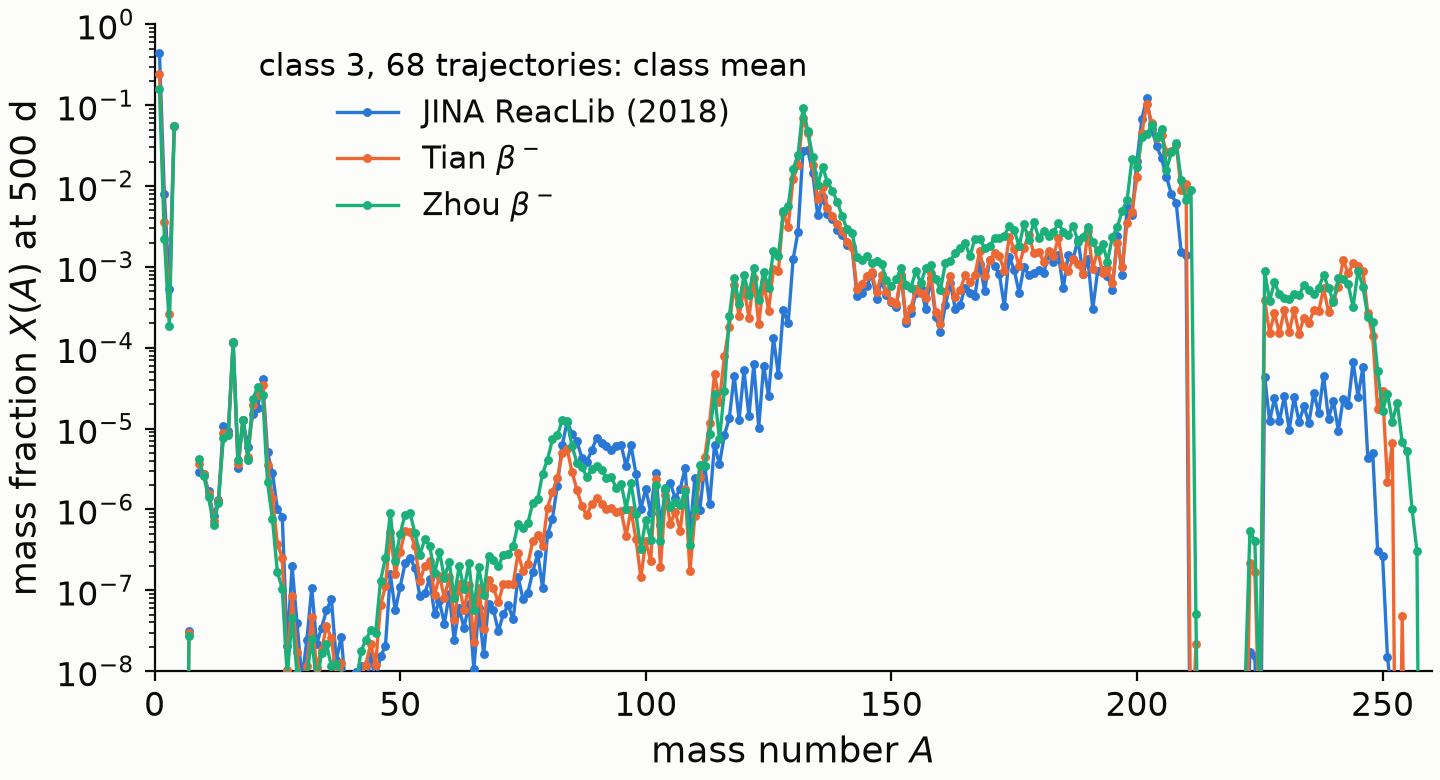
\includegraphics[width=0.5\textwidth]{Figures/abundances_class3.png}}\hfil
\subfloat[Class 4]{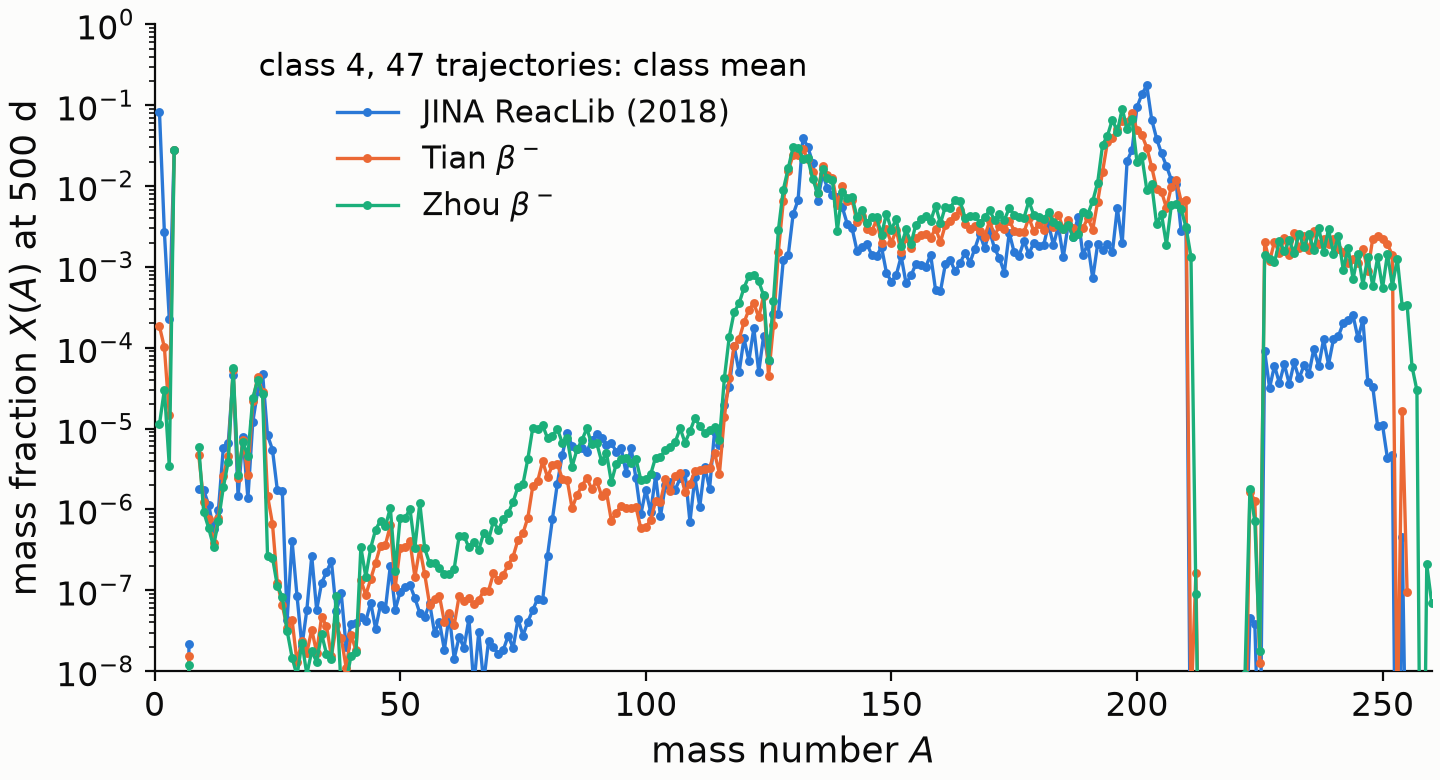
\includegraphics[width=0.5\textwidth]{Figures/abundances_class4.png}}%

\subfloat[Class 5]{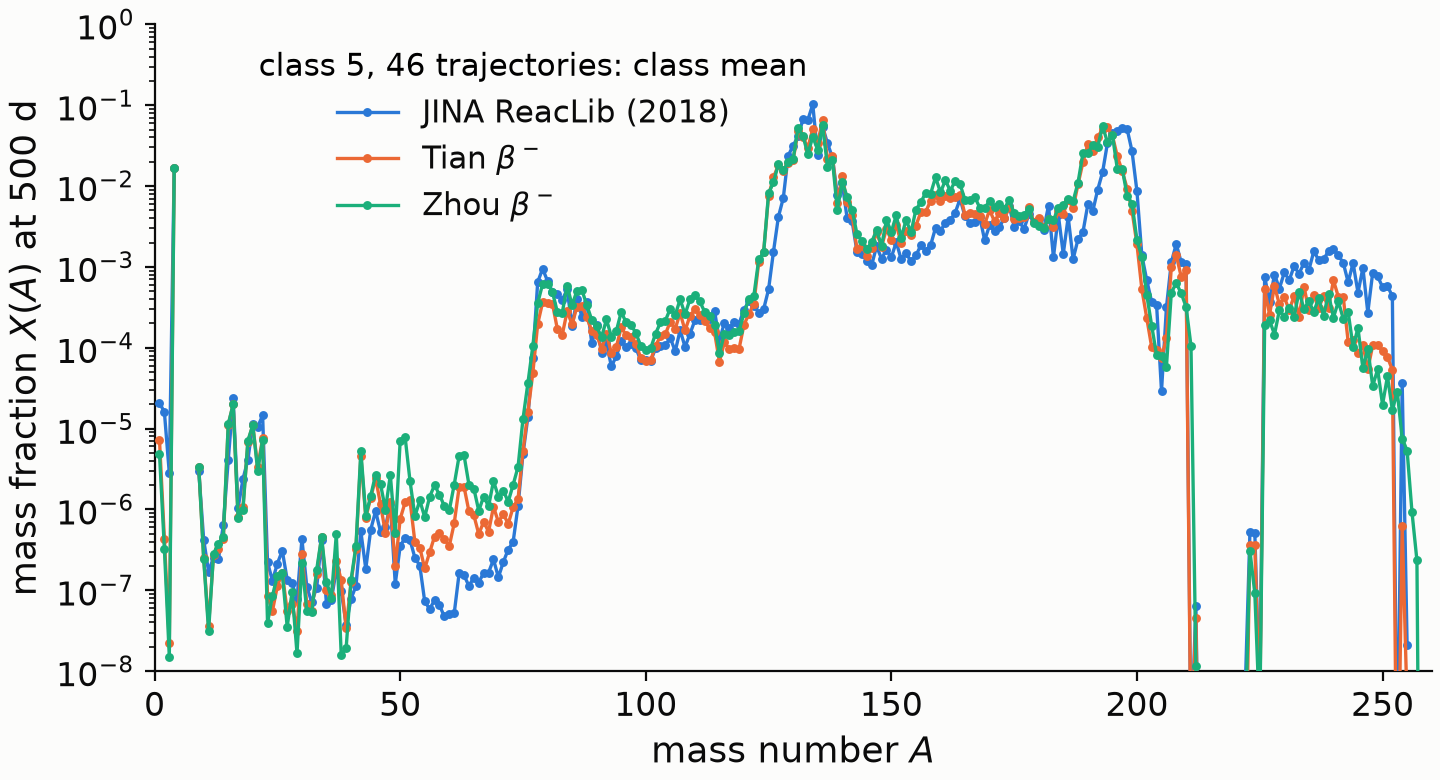
\includegraphics[width=0.5\textwidth]{Figures/abundances_class5.png}}
\caption{Final abundances of the five classes for the three prescriptions.}\label{fig:res_abund}\label{Abundances}
\end{figure}

Class~1 produces the first and second peaks and almost no lanthanides; its mean $X_{\rm LA}$ comes from its most neutron-rich trajectories.
Here the mass fractions of the three sets differ by at most about 0.02 in every range.
In the neutron-rich classes the prescription moves matter between three regions: the second peak ($A\approx120$--$140$), the third peak ($A\approx185$--$205$), and the rare earths and actinides.
Compared with the empirical sets, ReacLib keeps more matter in the second peak in classes~2 and~5 and more matter in the third peak in class~4, and in classes~3 and~4 an order of magnitude less of its matter reaches $A\geq210$.
In class~3 ReacLib leaves half of the mass at $A<70$, most of it hydrogen from the decay of free neutrons: the hydrogen mass fraction at 500\,d is 0.44, 0.24 and 0.16 for ReacLib, Tian and Zhou.
The lanthanide and actinide fraction follows the order ReacLib $<$ Tian $<$ Zhou in every class; over the whole ensemble its mean is 0.063, 0.097 and 0.119.

The $\beta^-$ rates of the closed-shell nuclei set how much matter accumulates in the peaks and how fast it moves past them~\cite{mumpower_impact_2016}, and most of these trends are consistent with one reading: compared with the two empirical formulae, FRDM+QRPA retains matter longer at the closed shells $N=82$ and $N=126$.
In the slower trajectories of classes~2 and~5 this leaves more matter in the second peak.
In the fast neutron-rich trajectories of classes~3 and~4, where the time available for the flow is short ($\tau\approx0.4$--$0.6\,\mathrm{ms}$), it keeps matter near $A\approx202$, so that less of it reaches $A\geq210$.
A slower flow also consumes fewer neutrons before freeze-out, which is consistent with the larger hydrogen fraction of ReacLib in classes~3 and~4.
In class~3 the matter that passes $N=126$ in the empirical sets reaches the fissioning nuclei, whose fragments would explain their richer second peak.
This reading rests on unmeasured half-lives, and it does not explain why ReacLib produces the most actinides in class~5.

In the slower trajectories of class~2, all three sets carry matter past $N=126$ (8--14\% of the mass ends at $A\geq210$), and the difference moves to the survival of the $A\geq240$ material.
There the clean comparison is between Tian and Zhou.
With identical $\alpha$ rates, Tian retains enough $A\geq240$ material to make fission a third of its released energy, whereas Zhou retains essentially none.
In no class does Zhou release more than $0.3\%$ of its energy by fission.
The budgets alone do not decide whether the flow in Zhou stops below $A\approx240$, or whether the $A\geq240$ material is destroyed during the decay to stability.
The enhanced odd-$A$ $\alpha$ series of Zhou in classes~2 and~4, which requires matter at $A\approx223$--$229$, and the 10\% of its mass that still ends at $A\geq210$ in class~2 are consistent with the first possibility.

Finally, since the opacity of r-process matter is controlled mainly by $X_{\rm LA}$ (Sec.~\ref{sec:opacity}), the prescription can also change the opacity of a given trajectory, making the empirical sets more opaque than ReacLib.

%------------------------------------------------------------------------------------------
\section{Bolometric light curves}\label{sec:res_lum}
%------------------------------------------------------------------------------------------

The light curves are computed with the one-zone model of Sec.~\ref{sec:onezone}, with the effective heating rates of this chapter as the source term.
Each trajectory is treated as a uniform sphere of mass $M_{\rm ej}=0.05\,M_\odot$ expanding with $v_{\rm ej}=v_\infty$, and its released heating $\dot\epsilon_x$ is converted into the effective heating $\dot\varepsilon=\sum_x f_x\dot\epsilon_x$.
Electrons, $\alpha$ particles and fission fragments thermalize according to the formula of Ref.~\cite{kasen_radioactive_2019},
\begin{align}\label{eq:res_fineff}
    f_\gamma=1-\exp(-t_\gamma^2/t^2),&\qquad t_\gamma=0.3\left(\frac{M_{\mathrm{ej}}}{0.01M_\odot}\right)^{1/2}\left(\frac{v_{\mathrm{ej}}}{0.2c}\right)^{-1}\mathrm d,\\
  f_e(t)=\left(1+\frac{t}{t_e}\right)^{-1},&\qquad t_e=12.9\left(\frac{M_{\mathrm{ej}}}{0.01M_\odot}\right)^{2/3}\left(\frac{v_{\mathrm{ej}}}{0.2c}\right)^{-2}\mathrm d,\\
    f_\alpha(t)=\left(1+\frac{t}{t_\alpha}\right)^{-\frac{3}{2}},&\qquad t_\alpha=3t_e,\\
    f_{\mathrm{fiss}}=\left(1+\frac{t}{t_{\mathrm{fiss}}}\right)^{-\frac{3}{2}},&\qquad t_{\mathrm{fiss}}=5t_e,
\end{align}

The luminosity is the solution of the one-zone equation for an arbitrary heating rate, Eq.~\ref{eq:kn_Lsol} for $t<t_c$.
For times $>t_c$ the luminosity is the solution of Eq.~\ref{eq:kn_Lsol_late}.
Where $t_c$ is defined in Eq.~\ref{eq:kn_tthin}.
For the opacity we use a grey opacity, constant in time, that depends on $Y_{e,0}$ through three bins (Sec.~\ref{sec:opacity}): $\kappa=10\,\mathrm{cm}^2\mathrm g^{-1}$ for $Y_{e,0}<0.25$ (lanthanide-rich matter), $\kappa=1\,\mathrm{cm}^2\mathrm g^{-1}$ for $0.25\leq Y_{e,0}<0.40$, and $\kappa=0.1\,\mathrm{cm}^2\mathrm g^{-1}$ for $Y_{e,0}\geq0.40$ (lanthanide-poor matter).
Classes~2--4 lie entirely in the first bin, class~5 in the first two, and class~1 in all three.

To calculate the light curve of a class we used $M_{ej}=0.05\,M_\odot$ of ejecta with the conditions of the class.
We used the mean heating and velocity of the group to calculate the luminosity.
However, the class curves are not predictions for a merger.
A real kilonova is the sum of components with different masses (Sec.~\ref{sec:res_merger}).
Here our aim is to show how the differences in the heating propagate to the light curve in each regime.


\subsection{Light curves of the classes}\label{sec:res_lum_results}

\begin{figure}[t]
  \centering
  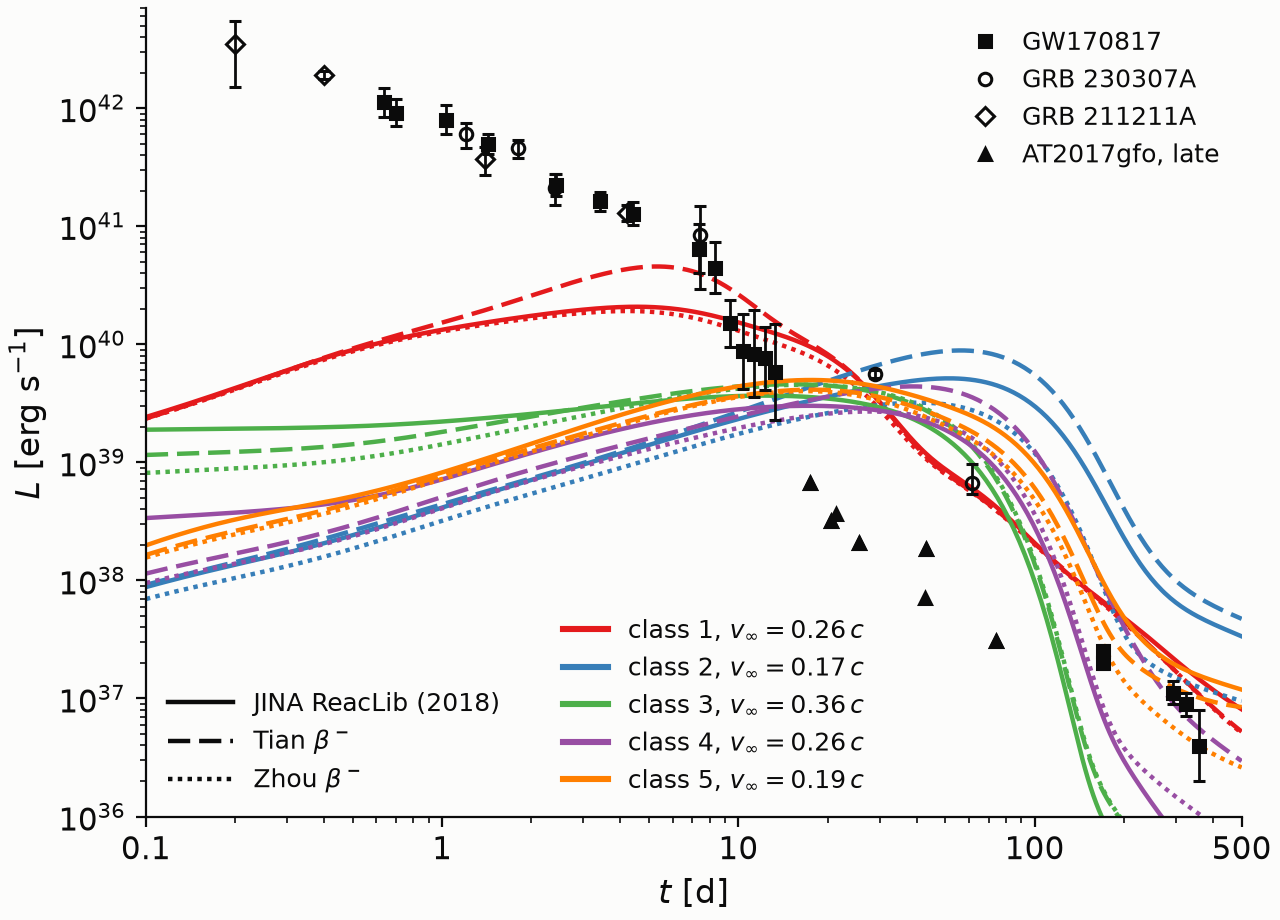
\includegraphics[width=0.85\textwidth]{Figures/luminosity_classes_Ye_v.png}
  \caption{Bolometric luminosity of $0.05\,M_\odot$ of ejecta with the conditions of each class, for the three prescriptions (solid: ReacLib, dashed: Tian, dotted: Zhou). The legend gives the mean velocity of each class. The symbols are the reconstructed bolometric luminosities of AT2017gfo (GW170817) with the triangles indicating the lower limits for the same kilonova~\cite{wu_fingerprints_2019,tanvir_emergence_2017,villar_spitzer_2018,kasliwal_spitzer_2021} and of the kilonovae of GRB~230307A~\cite{liu_constraint_2025,yang_lanthanide-rich_2024} and GRB~211211A~\cite{rastinejad_kilonova_2022}.}
  \label{fig:Luminosity}
\end{figure}

Figure~\ref{fig:Luminosity} shows the light curves of the five classes.
They fall into two groups.
Class~1, which contains the lanthanide-poor trajectories, is the brightest during the first week, with a peak of a few $10^{40}\,\mathrm{erg\,s^{-1}}$. 
The lanthanide-rich classes~2--5 are fainter at early times and peak later, at a few $10^{39}\,\mathrm{erg\,s^{-1}}$ after one to several weeks, because their larger opacity traps the radiation for longer. 
Between about one and six months class~2 is the brightest in all three sets, because $\alpha$ decay and fission release their energy over longer times than $\beta^-$ decay and thermalize more efficiently.
This is quite interesting because class~2 is also one of the most sensitive to the $\beta^{-}$ decay prescription. 

In the case of class~1 ReacLib and Zhou agree during the 500\,d.
The Tian curve is brighter around the peak but quickly disappears after about 20\,d.
So class~1 luminosity does not distinguish between prescriptions.
Class~2 on the other hand does.
Here the difference grows with time.
During the first days the three sets agree but near the peak they evolve in different ways.
At 500 d the difference between Tian and Zhou reaches a factor of a few.
ReacLib lies between the two.
Class~3 do not distinguish between prescriptions, similar as class~1 but with a rapidly decreasing luminosity due to the rapid expansion.
Class~4 is sensitive to the prescription but in a different way than class~2.
In class~2 Tian and reaclib do not differ that much compared with zhou but in class~4 is now Reaclib and zhou the ones that do not differ while tian predicts higher luminosities.
Class~5 has similar evolution to class~4 but with a modest sensitivity on the prescription. 

From the previous analysis we can say that the decay-rate prescription influences the bolometric light curve in a way that depends on the trajectory.
The size of the effect follows the weight of $\alpha$ decay and fission in the late heating.
In classes where $\beta^-$ decay dominates, classes~1, 3 and 5, the prescription is not relevant.
On the contrary, the prescription sensitivity is largest in classes~4 and~2, where one prescription heats by fission and another does not with an effect that in general grows with time.
Near the peak the effect is diluted by the $\beta^-$ heating common to the three sets.
After the peak the luminosity approaches the effective heating, $L\to M_{\rm ej}\dot\varepsilon$ (Eq.~\ref{eq:kn_late}), and the light curve inherits the full difference between the heating rates.
The imprint of the decay rates is therefore strongest in the late-time light curve, weeks to months after the merger, which is also the part that depends least on the opacity.

Figure~\ref{fig:Luminosity} also shows the bolometric luminosities of AT2017gfo and of the kilonovae that followed GRB~230307A and GRB~211211A.
The comparison only places the models on the observed scale, since each curve represents a single component of $0.05\,M_\odot$ with the conditions of one class.
During the first days all models are fainter than the observed transients by an order of magnitude or more.
This is expected, because the early emission of AT2017gfo requires fast, lanthanide-poor ejecta~\cite{villar_combined_2017} and the one-zone model underestimates the early luminosity.
Between one and two weeks class~1 is close to the luminosity of AT2017gfo, while between about 20 and 80\,d the models lie above the late-time points of AT2017gfo. 
